% !TEX root = ../thesis-example.tex
%
\chapter{Uncertainty Visualization for 2D Ultrasound}
\label{chap:cmvis}

Though there are many advantages of ultrasound imaging, such as being rather low-cost and real-time capable, the correct interpretation of B-mode images is a non-trivial task that requires a large amount of experience and training.
Even ultrasound experts sometimes struggle in performing an ultrasound-based diagnosis due to the presence of many different kinds of artifacts and it's non-homogeneous distribution of uncertainty.
In this chapter we present novel visualization techniques that augment the B-mode images with uncertainty information in real-time in order to support both ultrasound novices and expert users in gaining a better understanding of ultrasound.
Therefore, we build upon the previously introduced method of real-time confidence estimation for B-mode ultrasound images (cf. Chapter \ref{chap:cudacm}) and interpret these Confidence Maps as per-pixel uncertainty information, which we expose to the user using perceptual visualization techniques.
After a review on general uncertainty visualization techniques for medical applications, we discuss the clinical significance of our proposed system.
In total, we present three different visualization schemes for both educational and clinical applications and motivate the selection of visual variables to depict uncertainty in B-mode ultrasound images.
An extensive evaluation conducted with both ultrasound novices and expert clinicians demonstrates the usefulness of our techniques.
Parts of this work have been published in \CN.


\section{Uncertainty in Health Care and Medical Visualization}
\label{sec:cmvis:uncertainty-vis-techniques}
When \SYN{having} a comprehensive look at health care, the concept of uncertainty is ubiquitous throughout all levels.
However, since clinicians have been trained to make decisions and provide their patients with answers, many of them struggle to admit that their work is based on a plethora of input factors, each inducing an individual level of uncertainty, and thus their eventual findings rather represent the most likely interpretation than the \SYN{absolute truth}.

Han et al. investigate the different concepts and appearances of uncertainty in general health care using cancer treatment as example and derive a conceptual taxonomy in \cite{Han:2011:UncertaintyInHealthCare}.
They point out that a coherent concept of uncertainty in health care is missing and that multiple meanings and interpretations of that term are present, which are not necessarily distinguished from each other.
They conclude that uncertainty is actually a threefold concept which can originate either through probability, ambiguity or complexity with issues ranging from disease-centered to patient-centered ones.

While the paper of Han et al. analyzes the problem from the clinical perspective, Ristovski et al. focus on the various technical aspects and investigate the presence of uncertainty in medical visualization \cite{Ristovski:2014:UncertaintyInMedVis}.
As introduced in Section \ref{sec:background:vis:vispipeline}, the visualization pipeline ranges from the initial acquisition of data, over several data processing steps to the final rendering output.
Though each of these steps is subject to an individual level of uncertainty, the final rendering often shows the data as if it were the only possible truth.
However, it requires appropriate visualization to make the amount of uncertainty assessable to the clinician and thereby propagate the information back correctly to the clinical perspective as it was previously presented by Han et al.
For instance, Lundström et al. point out that a suboptimal setup of a transfer function during rendering can lead to a false classification of stenosis \cite{Lundstrom:2007:Animation}.

\begin{figure}[ht]
	\centering
	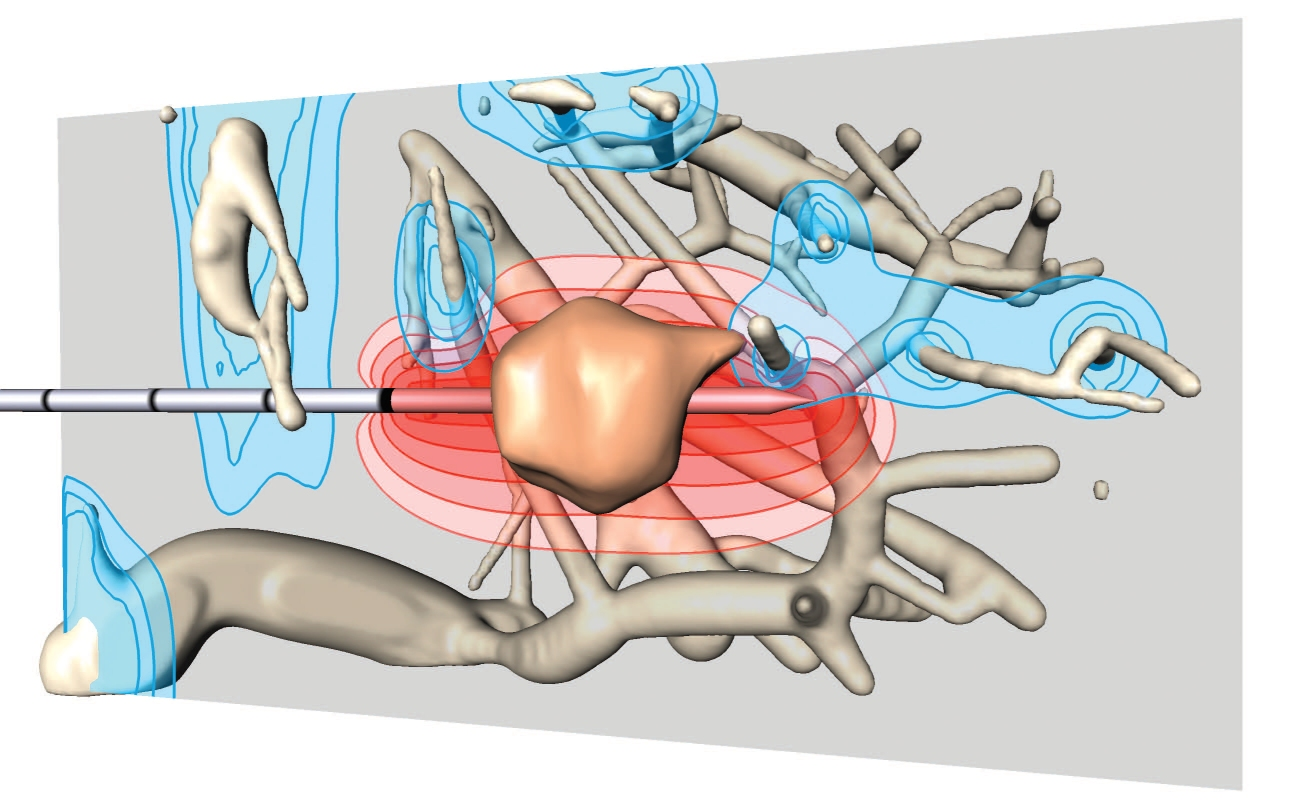
\includegraphics[width=0.75\linewidth]{figures/cmvis/rieder-rfablation.jpg}
	\caption{
		Uncertainty visualization of radio-frequency ablation zones as proposed by Rieder et al. \cite{Rieder:2011:AblationApproximation}.
	}
	\label{fig:cmvis:rieder-rfablation}
\end{figure}

The special setup in which medical visualization is used and its resulting requirements make it difficult to apply techniques from other domains, such as \cite{Pfaffelmoser:2011:VisualizingVariability, Pothkow:2011:PositionalUncertainty}, even though they use very similar data.
This may be one of the reasons why the body of literature on medical uncertainty visualization is rather shallow and the individual works are very application- and task-specific.
One such example is the uncertainty visualization technique of Rieder et al. proposed in the context of percutaneous radio-frequency ablation.
For this application, precise planning of the applicator placement is crucial in order to ensure that the malignant tissue is destroyed completely (cf. Figure \ref{fig:cmvis:rieder-rfablation}).
Their work is particularly noteworthy as they use their visualization for the optimization of a seven-dimensional optimization problem (five degrees of freedom for the placement of each needle plus two free simulation parameters) in three-dimensional space \cite{Rieder:2011:AblationApproximation}.
Another similar approach is the work of Brecheisen et al. exploring the parameter sensitivity in fiber tracking algorithms for DTI data \cite{Brecheisen:2009:ParameterSensitivy}.
Both techniques rely on interactive exploration by the user in order to cover the available parameter space.

\begin{figure}[ht]
	\centering
	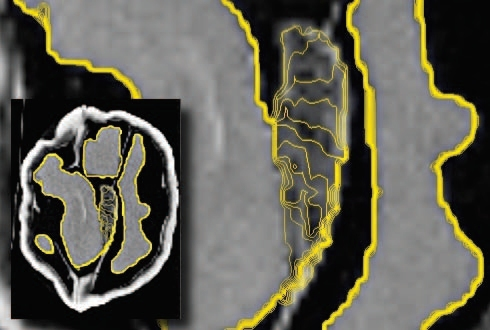
\includegraphics[height=4cm]{figures/cmvis/prassni-uncertainty1.jpg}
	\qquad
	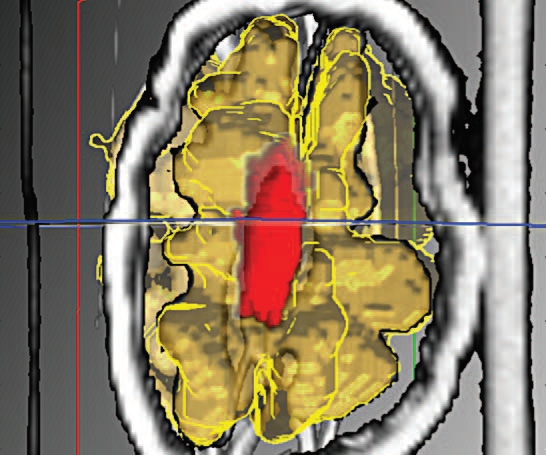
\includegraphics[height=4cm]{figures/cmvis/prassni-uncertainty2.jpg}
	\caption{
		Uncertainty visualization of segmentation algorithm results as proposed by Prassni et al. \cite{Prassni:2010:Uncertainty}.
	}
	\label{fig:cmvis:prassni-uncertainty}
\end{figure}

One example of providing feedback on the uncertainty present in medical imaging algorithms is the work of Praßni et al.
They propose a guided probabilistic volume segmentation technique for which they visualize the resulting uncertainty distribution using iso-lines and opacity modulation (cf. Figure \ref{fig:cmvis:prassni-uncertainty}).
As mentioned previously, it is crucial to expose information on the result quality to the clinician, since ultimately they have to decide on diagnosis and treatment.
The recent progress on ensemble visualizations \cite{Hao:2016:TemporalEnsembles, Obermaier:2014:FutureEnsemble, Rautenhaus:2015:EnsembleVisualization} could be influential for further progress in this direction.
In the medical domain such techniques can for instance be used to visualize the results of large random studies on medical imaging algorithms and thereby make them more accessible.




\section{Clinical Significance and Application}
\label{sec:cmvis:clinical-significance}

Compared to other anatomical medical imaging modalities such as CT or MRI, medical ultrasound exhibits several benefits, such as being comparatively cheap, portable and real-time capable.
It is therefore widely used in today's clinical practice, for instance for abdominal, pediatric, head and general vascular applications \cite{Noble:2011:Ultrasound}. 
However, acquiring a good image (e.g. in terms of high diagnostic value) is a non-trivial task due to the highly complex ultrasound image formation process (cf. Section \ref{sec:cudacm:us-image-formation}).
It is influenced by various physical imaging parameters such as frequency, focus, and depth, as well as by external factors such as probe positioning, probe pressure, patient positioning and patient breathing cycle \cite{Aldrich:2007:USPhysics}, and can yield a wide range of image artifacts \cite{Scanlan:1991:Artifacts}.
Furthermore, some target anatomies can not be directly reached but need to be scanned by circumventing strong reflectors such as bones, which prevent the acquisition of images underneath.
A classic example of such an anatomy are the kidneys, which can not be scanned from the back as they are then in the acoustic shadow of the spine reflecting almost all ultrasound waves.
Instead, sonographers perform kidney ultrasound through the abdomen, usually using the liver as an acoustic window since it has the best transmission properties of the surrounding anatomy.

\begin{figure}[ht]
	\centering
	\subfloat[]{
		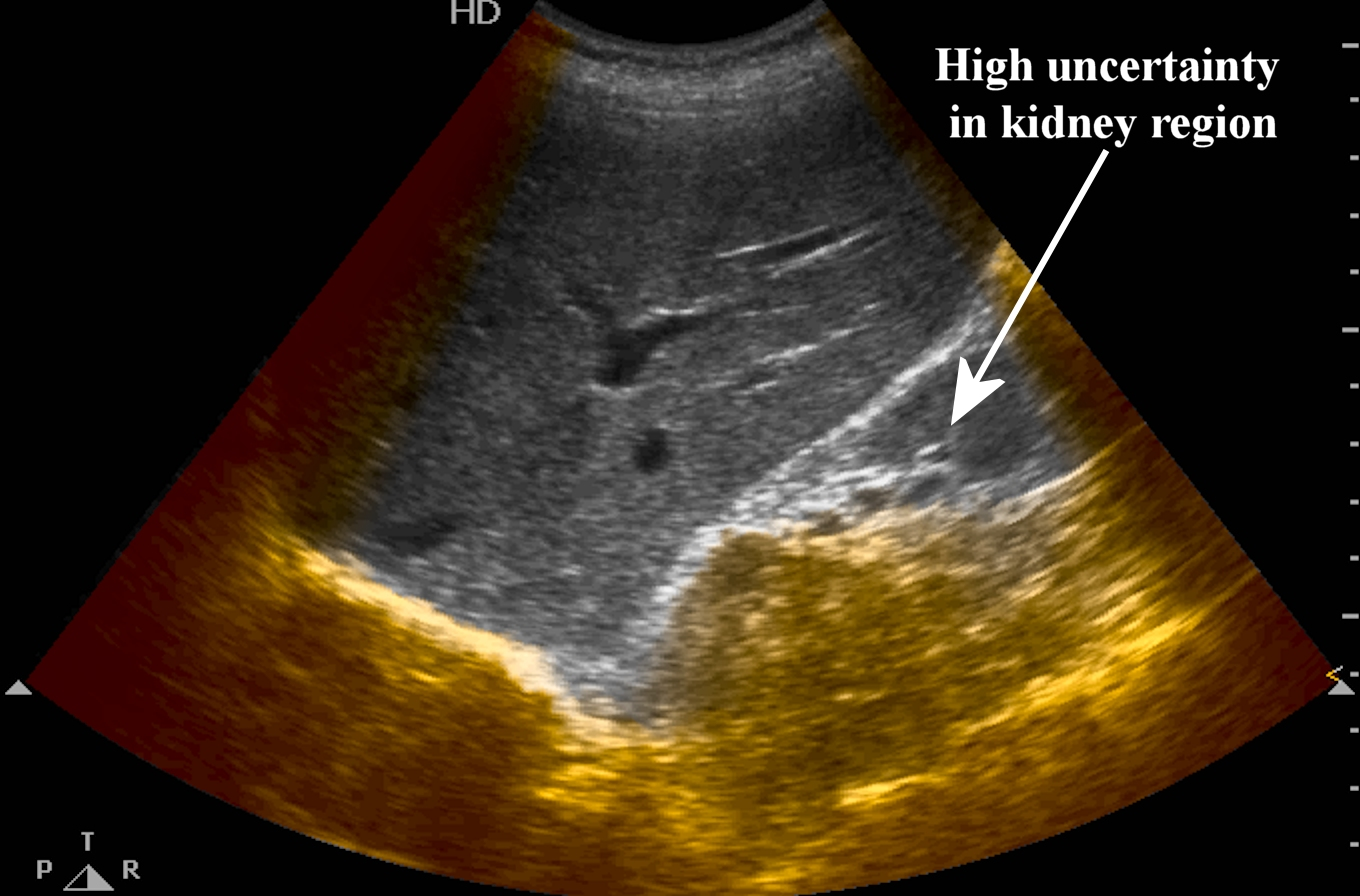
\includegraphics[width=0.42\linewidth]{figures/cmvis/liver_high_uncertainty.jpg}
	}	
	\qquad
	\subfloat[]{
		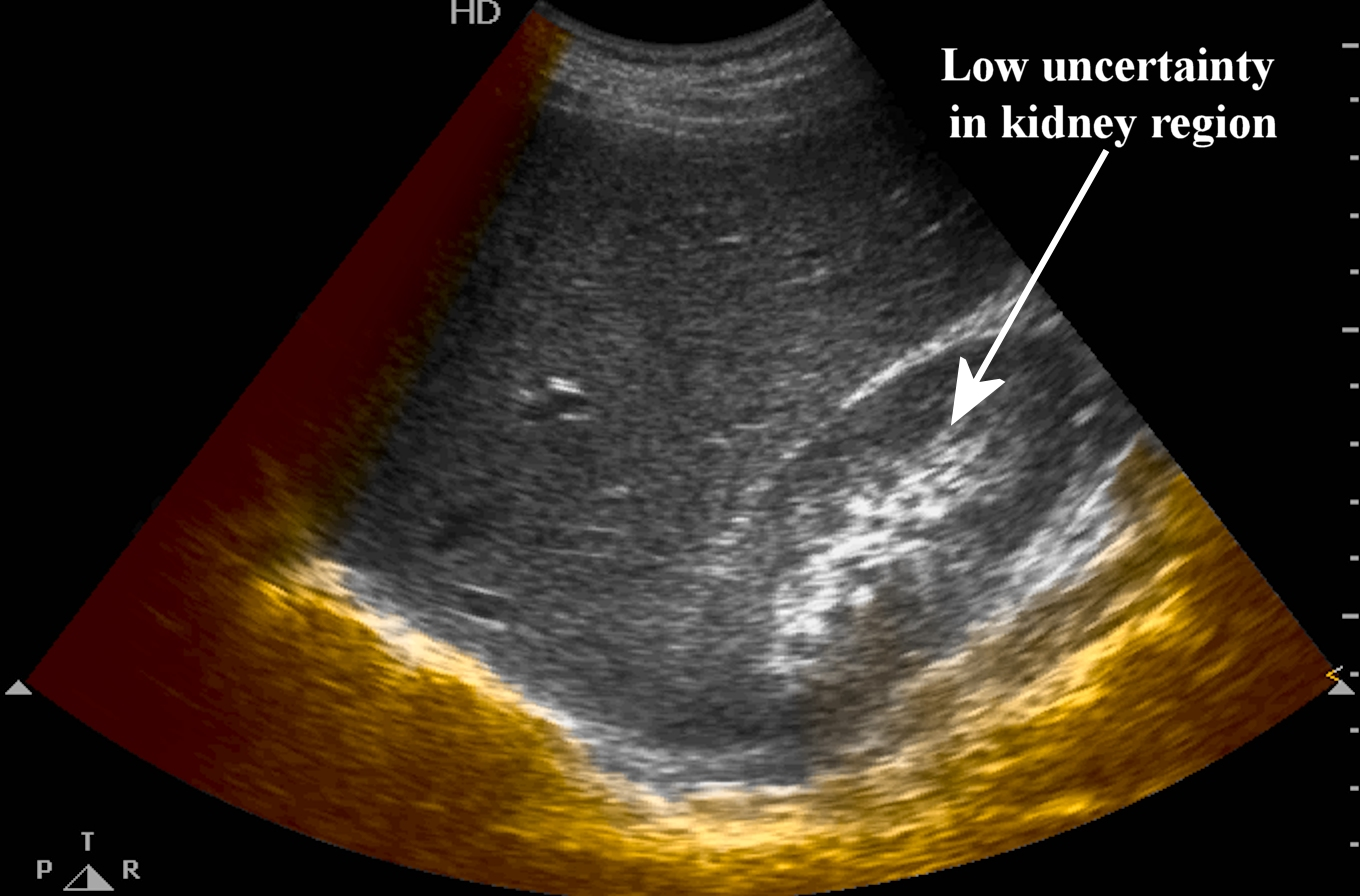
\includegraphics[width=0.42\linewidth]{figures/cmvis/liver_low_uncertainty.jpg}
	}
	\caption{
		\textbf{Kidney ultrasound using the liver as acoustic window} with applied uncertainty visualization using chroma as visual variables (cf. Section \ref{sec:cmvis:mapping-schemes}).
		A slight repositioning of the transducer results in a considerable increase of confidence in image (b) compared to (a).}
	\label{fig:cmvis:kidney_acoustic_window}
\end{figure}

Sonographers need to be aware of all these caveats of ultrasound imaging in order to correctly understand the image.
In particular medical trainees and ultrasound novices have difficulties in getting the right image needed for their clinical objectives since traditional ultrasound imaging does not provide a direct qualitative feedback on the image quality.
Already a slight repositioning of the transducer can yield a significantly better acoustic window and thus improve the image for the target anatomy (cf. Figure \ref{fig:cmvis:kidney_acoustic_window}).
Thus, training is an important aspect for medical students when learning ultrasound \cite{Butter:2007:UsTraining}.
In particular in trauma applications, where time is critical, the surgeon has to determine possible fractures and lesions as quickly as possible and has a minimal margin for error \cite{Knudtson:2004:TraumaSuite}.
With this motivation in mind, we developed our work with the aim to support both medical students in learning sonography as well as expert clinicians for a more quick and intuitive interpretation of ultrasound images by providing an interactive feedback on the image quality and uncertainty distribution.


\section{Selection of Visual Variables}
\label{sec:cmvis:selection-visual-variables}

Essentially, we target two different applications with our work:
On the one hand, we are convinced that exposing uncertainty information to ultrasound novices and trainees helps them to better understand the complex ultrasound image formation process.
At the same time, we also expect expert sonographers to benefit from uncertainty visualization as the additional information may improve the diagnostic value of the image.
Regarding these two target applications, we yield the following requirements for ultrasound uncertainty visualization schemes.
\begin{my_list_item}
	\item 
		The uncertainty information should be fused directly into the original B-mode sequence. Thus, both the spatial and the temporal domain are fixed.
		
	\item
		The primary information in the uncertainty maps are not the exact per-pixel uncertainty values but the distribution of the uncertainty with respect to the anatomy (cf. Section \ref{sec:cudacm:cm}).
		
	\item
		For educational applications, the uncertainty distribution in the image should be easily and intuitively perceivable. Even small changes in the uncertainty distribution should be clearly observable when repositioning the ultrasound probe in order to maximize the learning effect.
		
	\item
		For clinical applications, the diagnostic information in the B-mode image must not be impaired. Thus, the original image intensities should be preserved as good as possible and no image regions should be occluded.
\end{my_list_item}
Given these requirements for our uncertainty visualization, the number of viable visual variables for depicting the uncertainty information is limited.

One traditional technique is the usage of glyphs for depicting uncertainty, with error bars in 1D visualization being the classic example.
Glyphs have the advantage of offering a large number of visual variables that can be used to alter their appearance.
For instance, MacEachren et al. evaluate 11 different mappings of uncertainty to point glyphs \cite{MacEachren:2012:VisualSemiotics}.
Glyphs excel in depicting uncertainty when used in sparse layouts allowing the observer to individually focus on single glyphs in order to read their information.
However, this does not work well for our application where the goal is to visualize the distribution of a dense 2D scalar field.
Although dense glyph fields have also been successfully used for depicting global information \cite{Kindlman:2006:GlyphPacking, Borgo:2012:GlyphVisualization}, we do not consider them for our work since early experiments did not show promising results.
The work of Sanyal et al. supports this fact as their experiments showed that in many uncertainty related tasks on 2D data sets the different glyph mappings perform significantly worse than surface color mapping \cite{Sanyal:2009:UncertaintyVis}.
Furthermore, adding glyphs to the B-mode image would occlude the original ultrasound image, which is undesirable for clinical applications.

One intriguing approach is to extend the 2D data to the third dimension and map uncertainty to the Z axis in a 3D rendering \cite{Brown:2004:VibrationVis, Kao:2001:Eosvis}.
While this may be a valid method for applications such as geospatial visualization, it can not be applied to our use case since, due to the 2D projection of a 3D scene, it requires the user to interact with the camera to get the full information.
Furthermore, as mentioned above, the spatial domain of our visualization is fixed as clinicians expect a 2D image when performing 2D B-mode ultrasound.

Another approach is to exploit the spatial domain for depicting uncertainty, for instance through animations, animated jittering or probabilistic animation \cite{Brown:2004:VibrationVis, Lundstrom:2007:Animation}.
However, since we are working with real-time ultrasound sequences, the temporal domain is fixed and such approaches are not applicable.
\TODO{extend the last two paragraphs/this section}


\section{Visualization Schemes}
\label{sec:cmvis:mapping-schemes}

Given these considerations and the particular requirements of our intended uncertainty visualization, we selected the visual variables of color and texture.
They both do not affect the spatial and temporal image domain and are very powerful and intuitive for expressing general uncertainty \cite{MacEachren:2012:VisualSemiotics}.
In total, we propose three different uncertainty mapping techniques for the two applications, which we will discuss in detail in the following sections.
Since both the B-mode image and the uncertainty map are in the same image domain, no coordinate transformation is necessary and the mapping techniques are focused on the optical properties.

\begin{figure}[ht]
	\centering
	\begin{tikzpicture}[%
	schritt/.style={%
		schritt-base, minimum height=8mm, minimum width=22mm%
	},%
	entity/.style={%
		entity-base, minimum height=8mm, minimum width=26mm%
	}, %
	portL/.style={
		font=\sffamily\scriptsize, outer xsep=1mm,
		align=left, anchor=west,
	},
	portR/.style={
		font=\sffamily\scriptsize, outer xsep=1mm,
		align=right, anchor=east,
	},
	node distance=5mm and 7mm%
]%
	\renewcommand{\arraystretch}{1.0}		% set vertical line padding to factor 1.0
	\setlength{\tabcolsep}{4pt}				% set the column separation (6pt is default)
	
	\node (usframe) [entity] {
		\begin{tabular}{cc}
			\parbox[c]{8mm}{\pgfimage[interpolate=true, height=0.5cm]{figures/uscompounding/im50.png}} & US Frame
		\end{tabular}
	};
	\node (registration) [schritt, below left=of usframe] {Registration};
	\node (clustering) [schritt, below=of registration] {Clustering / \\ Partitioning};
	
	\node (gencm) [schritt, below right=of usframe] {Compute \\ Uncertainty};
	\node (cluster) [entity, below=of clustering] {
		\begin{tabular}{cc}
% 				\parbox[c]{8mm}{\pgfimage[interpolate=true, height=0.5cm]{figures/uscompounding/cluster.png}} & Cluster
			\multirow{2}{8mm}{\pgfimage[interpolate=true, height=0.5cm]{figures/uscompounding/cluster.png}}
				& Batch of \\ & US Frames
		\end{tabular}
	};
	
	\node (cm) [entity, below=of gencm, yshift=-13.5mm] {
		\begin{tabular}{cc}
			\multirow{2}{8mm}{\pgfimage[interpolate=true, height=0.5cm]{figures/uscompounding/cm50.png}}
				& Uncertainty \\ & Map
		\end{tabular}
		};
		
	\node (compcluster) [schritt, rectangle split, rectangle split parts=2, below right=of cluster] {
		\textbf{Incremental Compounding} 
		\nodepart{two} \phantom{pb}\\\phantom{pb}
%		\phantom{pb} Batch of Frames \phantom{pb} \\
%		\phantom{pb} Accumulated Frames \phantom{pb}
	};
	\PORT{1L1}{($ (compcluster.two west) + (0, 1.5mm) $)}{MyColor2}{node[portL] {$I_i$\phantom{pb}}}
	\PORT{1L2}{($ (compcluster.two west) - (0, 1.5mm) $)}{MyColor4}{node[portL] {$I_{i-1}$\phantom{pb}}}
	\PORT{1R1}{($ (compcluster.two east) + (0, 1.5mm) $)}{MyColor2}{node[portR] {\phantom{pb} $U_i$}}
	\PORT{1R2}{($ (compcluster.two east) - (0, 1.5mm) $)}{MyColor4}{node[portR] {\phantom{pb} $U_{i-1}$}}
	\PORT{1S1}{($ (compcluster.south) + (1.5mm, 0mm) $)}{MyColor2}{}
	\PORT{1S2}{($ (compcluster.south) - (1.5mm, 0mm) $)}{MyColor2}{}
	
	\node (compimg) [entity, below right=of compcluster, xshift=-10mm, yshift=-5mm] {
		\begin{tabular}{cc}
			\multirow{2}{6mm}{\pgfimage[interpolate=true, height=0.5cm]{figures/uscompounding/cube.png}}
				& Compounded \\ & US Volume
		\end{tabular}
	};
	\node (compcm) [entity, below left=of compcluster, xshift=10mm, yshift=-5.75mm] {
		\begin{tabular}{cc}
			\multirow{2}{6mm}{\pgfimage[interpolate=true, height=0.5cm]{figures/uscompounding/cube.png}}
				& Compounded \\ & Uncertainty Volume
		\end{tabular}
	};
	
	\node (transducer) [above left=of usframe, yshift=5mm, xshift=5mm] {
		\pgfimage[interpolate=true, height=1.5cm]{figures/uscompounding/transducer.png}
	};
	
	\node (vis) [right=of compimg, yshift=0cm, xshift=15mm] {
		\pgfimage[interpolate=true, height=1.5cm]{figures/uscompounding/computer.png}
	};
	
	
	\begin{pgfonlayer}{background}
		\draw[pfeil] (usframe.east)  -| (gencm.north);
		\draw[pfeil] (usframe.west) -| (registration.north);
		
		\path
			(registration) edge[pfeil] (clustering)
			(clustering) edge[pfeil] (cluster)
			
			(gencm) edge[pfeil] (cm)
			;
		
		\draw[pfeil, shorten >=0.5mm] (cluster.south) |- (1L1);
		\draw[pfeil, shorten >=0.5mm] (cm.south) |- (1R1);
		
		\draw[pfeil] (1S1) |- (compimg.west);
		\draw[pfeil] (1S2) |- (compcm.east);
	
		\draw[pfeil, color=MyColor4, shorten >=0.5mm] (compimg.north) |- (1R2);
		\draw[pfeil, color=MyColor4, shorten >=0.5mm] (compcm.north) |- (1L2);
	
		\draw [pfeil] 
			(transducer) to [bend left=35] 
				node [align=center, font=\scriptsize, midway, above, xshift=12mm, yshift=-2mm] {Stream of \\ Tracked US Frames} 
			(usframe.north);
	
		\draw [pfeil] 
			(compimg.east) to [bend left=0] 
				node [align=center, font=\scriptsize, midway, above] {Interactive \\ Visualization} 
			(vis.west);
	\end{pgfonlayer}{background}

\end{tikzpicture}
	\caption{
		\textbf{Schematic diagram} of the different proposed uncertainty visualization schemes.
		Given the original B-mode ultrasound image $I$, we compute its Confidence Map $CM$ and a Gaussian blurred version $G_\sigma$. 
		The uncertainty map $U$ is derived from $CM$ by inverse linear mapping (cf. Equation \ref{eq:cmvis:u-from-cm}). 
		For the color overlay and the uncertainty mapping to chroma, we compute a derived uncertainty measure $U'$ using a transfer function. 
		Finally, the uncertainty information is fused into the original ultrasound image using one of the three visualization schemes.
	}
	\label{fig:cmvis:schematic-diagram}
\end{figure}

As illustrated in Figure \ref{fig:cmvis:schematic-diagram}, all proposed mapping schemes start with the original B-mode ultrasound image $I$, for which we compute the corresponding Confidence Map.
We assume it to be inversely related to the amount of uncertainty in the image, more precisely to it's facets of accuracy, precision and credibility.
Thus, we obtain the per-pixel uncertainty information $U$ by applying a direct inverse linear mapping
\begin{equation}
	\label{eq:cmvis:u-from-cm}
	U(x) := 1 - CM(x),
\end{equation}
where $CM(x) \in [0,1]$ is the confidence map value at pixel $x$ in the image domain.


\subsection{Uncertainty as Color Overlay}
\label{sec:cmvis:color-overlay}
For educational applications, the focus of the visualization should be on the uncertainty information and even small changes in the distribution should be clearly distinguishable by the observer.
At the same time, the corresponding ultrasound B-mode image should be shown as anatomical reference in order to allow for an understanding of the connection between image features and their effects on the uncertainty.
Therefore, we combine the visual variables of hue and value in our proposed color overlay scheme (cf. Figure \ref{fig:cmvis:schematic-diagram}).
Compared to the other presented mapping schemes, the combination of the two visual variables makes even subtle changes of uncertainty visible to the observer.
We deem this an important feature to teach ultrasound novices the caveats of the ultrasound image formation process.


As previously introduced, for each pixel $x$, let $U(x)$ be its uncertainty value and $I(x)$ be its original B-mode intensity.
Since the color overlay is a very obtrusive mapping scheme, we use a transfer function to apply a thresholding to the uncertainty measure and define the derived uncertainty as $U'(x) := \max \left( 0, \, 2 U(x) - 1 \right)$.
Using this derived measure instead of the original $U(x)$ avoids overlaying regions of negligible uncertainty.
We first generate the color overlay in HSV color space as
\begin{equation}
	C(x)_{HSV} := \left( H, U'(x), V \right),
\end{equation}
with constant hue $H \in [0, 1]$ and constant value $V \in [0, 1]$.
We chose a bright orange color with $H = 0.15$ and $V = 0.8$ to avoid lowering the contrast to Doppler ultrasound utilizing the colors blue and red.
In a second step, we linearly mix the color overlay transformed to RGB color space with the original B-mode to yield the final pixel color 
\begin{equation}
	O(x) := U'(x) \cdot C_{RGB}(x) + \left( 1 - U'(x) \right) \cdot I(x).
\end{equation}
Figure \ref{fig:cmvis:vis-color-overlay} shows the uncertainty color overlay applied to two different abdominal ultrasound images.

\begin{figure}[ht]
	\centering
	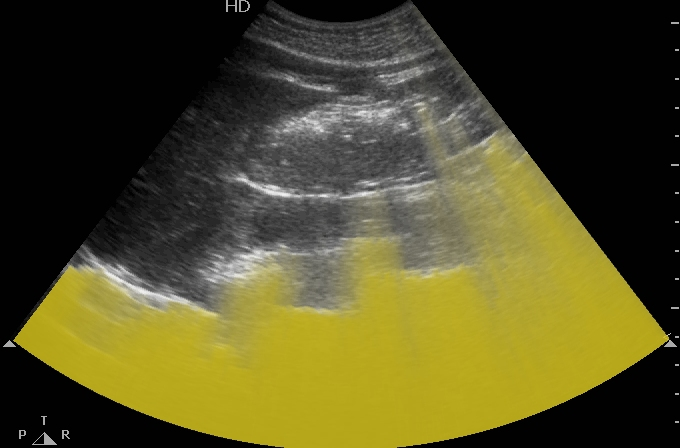
\includegraphics[width=0.42\linewidth]{figures/cmvis/color-overlay-100.jpg}
	\qquad
	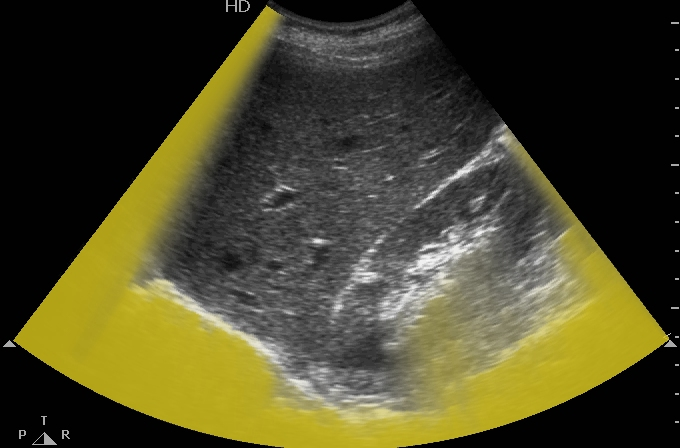
\includegraphics[width=0.42\linewidth]{figures/cmvis/color-overlay-300.jpg}
	\caption{
		Illustration of the color overlay mapping scheme.
		The high contrast yellow overlay allows for an \SYN{clear investigation} of the signal loss effects in ultrasound.
	}
	\label{fig:cmvis:vis-color-overlay}
\end{figure}

Since the original B-mode intensities are altered in this mapping scheme, we propose to use it only for educational purposes to give ultrasound novices a better understanding of the image formation process, but do not consider it for clinical usage.
Furthermore, the color overlay also partially occludes the original ultrasound intensities.
Although image regions of low confidence may not be reliable enough for diagnosis, they still contain structural information, which can help the sonographer in navigating towards the correct anatomy and optimizing the acoustic window. 
Thus, hiding these parts completely is disadvantageous for clinical usage, which was later also confirmed by some candidates during our evaluation (cf. Section \ref{sec:cmvis:evaluation}).
Therefore, we additionally propose two alternative mapping schemes maintaining structural information also in highly unreliable regions.



\subsection{Uncertainty Mapping to Chroma}
\label{sec:cmvis:mapping-to-chroma}

For clinical applications, we propose additional uncertainty visualization schemes that maintain the structural information in the ultrasound B-mode image also in unreliable regions.
Similar to the color overlay, uncertainty mapping to chroma also uses color to depict uncertainty but uses chroma as visual variable.

In order to preserve the original ultrasound image's diagnostic value, we need to ensure that the perceived intensity remains the same when augmenting the image with uncertainty information.
Therefore, we perform the chroma modification in the perceptually uniform CIE L*C*h* color space, the polar coordinate derivative of the CIE L*a*b* color model \cite{Plataniotis:2000:ColorImageProcessing}.

As illustrated in Figure \ref{fig:cmvis:schematic-diagram}, we compute the derived uncertainty from the original Confidence Map as $U'(x) := \max \left( 0, \, \frac{3 U(x)}{2} - \frac12 \right)$ to again avoid coloring regions with negligible uncertainty.
The final pixel color in L*C*h* space is given by
\begin{equation}
	C(x)_{L^*C^*h^*} := \big( I(x)_{L^*}, U'(x), H \big),
\end{equation}
where $I(x)_{L^*}$ is B-Mode intensity transformed to to $L^*$ space and $H = 0.23$ is a bright orange.
Again, we chose bright orange as hue for depicting uncertainty to avoid lowering the contrast to Doppler ultrasound.
Sample images are shown in Figure \ref{fig:cmvis:vis-chroma}.

\begin{figure}[ht]
	\centering
	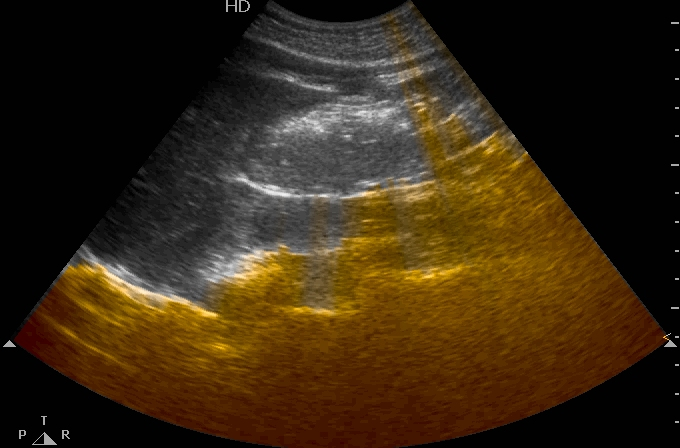
\includegraphics[width=0.42\linewidth]{figures/cmvis/chroma-100.jpg}
	\qquad
	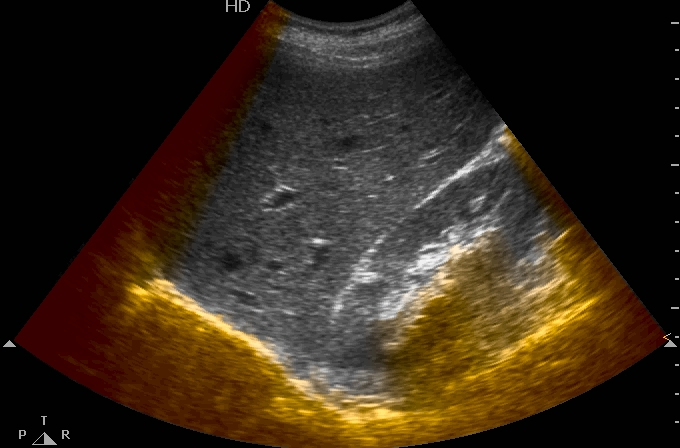
\includegraphics[width=0.42\linewidth]{figures/cmvis/chroma-300.jpg}
	\caption{
		Illustration of the chroma mapping scheme.
		Unreliable regions in the image are depicted with an orange overlay.
		Since the color transformation is applied in the perceptually uniform CIE L*C*h* color space, the perceived pixel intensity is maintained.
	}
	\label{fig:cmvis:vis-chroma}
\end{figure}


\subsection{Uncertainty Mapping to Fuzziness}

Many clinicians prefer to look at gray scale ultrasound images as they have been trained to do so.
Since texture is a very effective visual variable that keeps the spatial, temporal and color domain of the original image, we selected it as third visualization scheme for real-time B-mode ultrasound.
More precisely, we use the visual cue of fuzziness to map the uncertainty information.
Therefore, we fuse the ultrasound image with its uncertainty map such that regions of low uncertainty appear sharp and regions of high uncertainty appear fuzzy.
As a matter of fact, according to MacEachren et al., this visual variable is also the most intuitive to represent uncertainty \cite{MacEachren:2012:VisualSemiotics}.

Our proposed uncertainty mapping to fuzziness combines a slight Gaussian blur of the original ultrasound image with its unsharp mask (subtraction of the blurred image from the original image).
As illustrated in Figure \ref{fig:cmvis:schematic-diagram} we compute the confidence map of the original image and apply Equation \ref{eq:cmvis:u-from-cm} to obtain the uncertainty value $U(x)$ for each pixel $x$.
Since this is a diverging mapping scheme, where regions with high uncertainty will be blurred, and regions of low uncertainty will be sharpened, we can directly use $U(x)$ and do not need to compute a derived uncertainty measure.
We compute a Gaussian filtered version of the original image and combine the two to yield the final pixel value $F(x)$ as
\begin{equation}
	F(x) = U(x) G_\sigma(x) + \big( (1-U(x)) \cdot (2I(x) - G_\sigma(x)) \big),
\end{equation}
where $I(x)$ is the original ultrasound intensity and $G_\sigma(x)$ the corresponding intensity in the Gaussian with parameter $\sigma$.
We choose $\sigma = 2.5$ to limit the blurring to a tolerable amount but still yield the effect of perceived differences in fuzziness.
An exemplary result can be seen in Figure \ref{fig:cmvis:vis-fuzziness}.

\begin{figure}[ht]
	\centering
	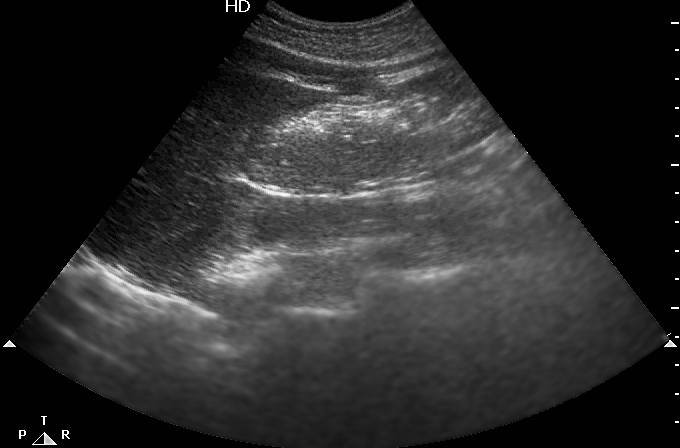
\includegraphics[width=0.42\linewidth]{figures/cmvis/fuzzy-100.jpg}
	\qquad
	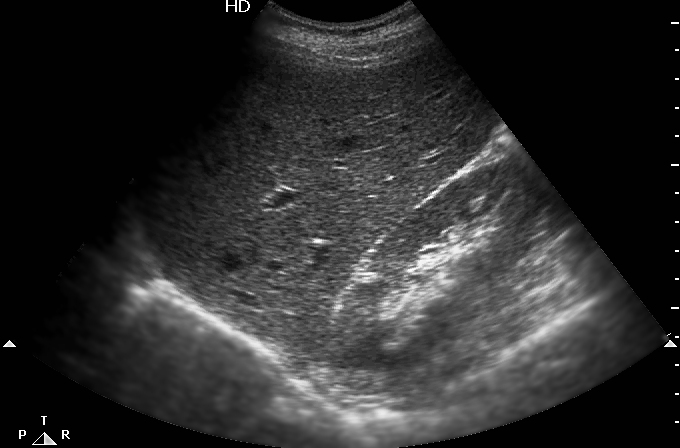
\includegraphics[width=0.42\linewidth]{figures/cmvis/fuzzy-300.jpg}
	\caption{
		Illustration of the fuzziness mapping scheme.
		Unreliable regions in the image are blurred while reliable regions are sharpened through unsharp masking.
		Especially in video sequences this provides a very strong perceptual cue for uncertainty while at the same time maintaining the ultrasound image in its original gray scale color domain.
	}
	\label{fig:cmvis:vis-fuzziness}
\end{figure}

It should be noted that this mapping scheme certainly alters the original B-mode image in a way that may reduce the amount of original information in regions of high uncertainty.
However, discussions with clinicians showed that they nevertheless like uncertainty mapping to fuzziness and appreciate the intuitiveness of the visual variable.
Our evaluation results in Section \ref{sec:cmvis:evaluation} underline this fact.



\section{Results and Evaluation}
\label{sec:cmvis:evaluation}

We performed the evaluation of the proposed methods independently for the two target applications.
Therefore, we implemented a fully working reference system using an Ultrasonix RP (Analogic Corporation, Peabody, MA, USA) ultrasound device for the acquisition of images.
Using OpenIGTLink \cite{Tokuda:2009:Openigtlink}, we stream the ultrasound frames and imaging parameters to a standard workstation where our computation framework performs the necessary processing steps before eventually routing the fused image back to the ultrasound device's display.
The processing pipeline is implemented in the CAMPVis framework \cite{SchulteZuBerge:2014:CAMPVis} and entirely executed on the GPU using both CUDA (solving of Equation \ref{cmvis:eq:cm-system}) and OpenGL/GLSL (all other processing steps) in order to achieve optimal performance.
After acquiring the B-mode image, we perform a Gaussian filtering as well as a resampling. 
Gaussian filtering is required in order to remove high-frequency noise as well as to allow for our uncertainty mapping to fuzziness.
We perform the downsampling to speed up the computation of the Confidence Maps and achieve better convergence (cf. Chapter \ref{chap:cudacm}). 
For our experiment setup we used a 0.5 scaling factor and a smoothing factor $\sigma$ of $2.5$.
Finally, one of the discussed uncertainty visualization schemes is applied and the rectilinear B-mode image in polar coordinates is scan converted to Cartesian coordinates using the known probe geometry and dynamically queried imaging parameters.

\subsection{User Study with Ultrasound Novices}

In a first user study we evaluated the educational value of our proposed system.
We equipped our ultrasound machine with an Ultrasonix C5-2/60 convex abdominal transducer and asked ultrasound novices to locate different structurally deep anatomies in a CIRS abdominal phantom while using our uncertainty visualization techniques.
In total we interviewed 13 medical students, which all had very limited experience with ultrasound (average of $5.6$ performed ultrasound examinations, minimum 0, maximum 20).

\begin{table}[th]
	\centering
	\begin{tabu} to 0.9\linewidth {>{\bfseries}m{40mm} C C C}
		\toprule
		& \bfseries Left Kidney & \bfseries Right Kidney & \bfseries Portal Vein \\
		&           \multicolumn{3}{c}{Average Time \emph{(seconds)}}            \\ \midrule
		Original B-Mode   & $6.73 \pm 4.3$        & $4.96 \pm 1.6$         & $4.78 \pm 1.2$        \\ \midrule
		Color Overlay     & $4.74 \pm 3.8$        & $4.26 \pm 1.5$         & $3.30 \pm 1.7$        \\
		Chroma Mapping    & $4.19 \pm 2.3$        & $3.42 \pm 1.8$         & $3.44 \pm 1.5$        \\
		Fuzziness Mapping & $3.49 \pm 3.9$        & $3.15 \pm 0.7$         & $2.67 \pm 1.1$        \\ \bottomrule
	\end{tabu}
	\caption{
		Quantitative evaluation results of our user study with ultrasound novices.
		The table shows the average time \emph{(seconds)} required to optimize the view on target anatomies (aggregated results from 9 of the 13 users, since not all acquisitions were complete).
		With enabled uncertainty visualization, the users managed to decide faster when they had a good view on the target anatomy than with the plain B-mode image.
	}
	\label{tbl:cmvis:timing-results}
\end{table}

For a quantitative evaluation, we recorded the acquisitions and measured the time the users required to optimize the view on anatomical targets.
After giving the participants some time to familiarize themselves with the phantom anatomy, we asked them to find an optimal view onto the vessel targets in the left and right kidney, as well as onto the portal vein.
We then measured the required time to optimize the view for each visualization scheme by counting the number of frames between the first frame where the target anatomy was in the field of view until the frame where the student defined the view as optimal in their personal opinion.
To avoid biasing the results, we shuffled the order of the visualizations for each user.
While the results in Table \ref{tbl:cmvis:timing-results} show no significant differences between color overlay and chroma mapping, the time needed with fuzziness mapping is consistently lower (in average 0.79 seconds) than with the one of other two mapping schemes.
Furthermore, the students performed significantly worse (in average 1.86 seconds longer) with only the original B-mode image compared to all of our proposed visualization schemes, which supports our idea that visualizing uncertainty helps the user in interactively assessing the quality of the acquired ultrasound image.

\begin{figure}[ht]
	\centering
	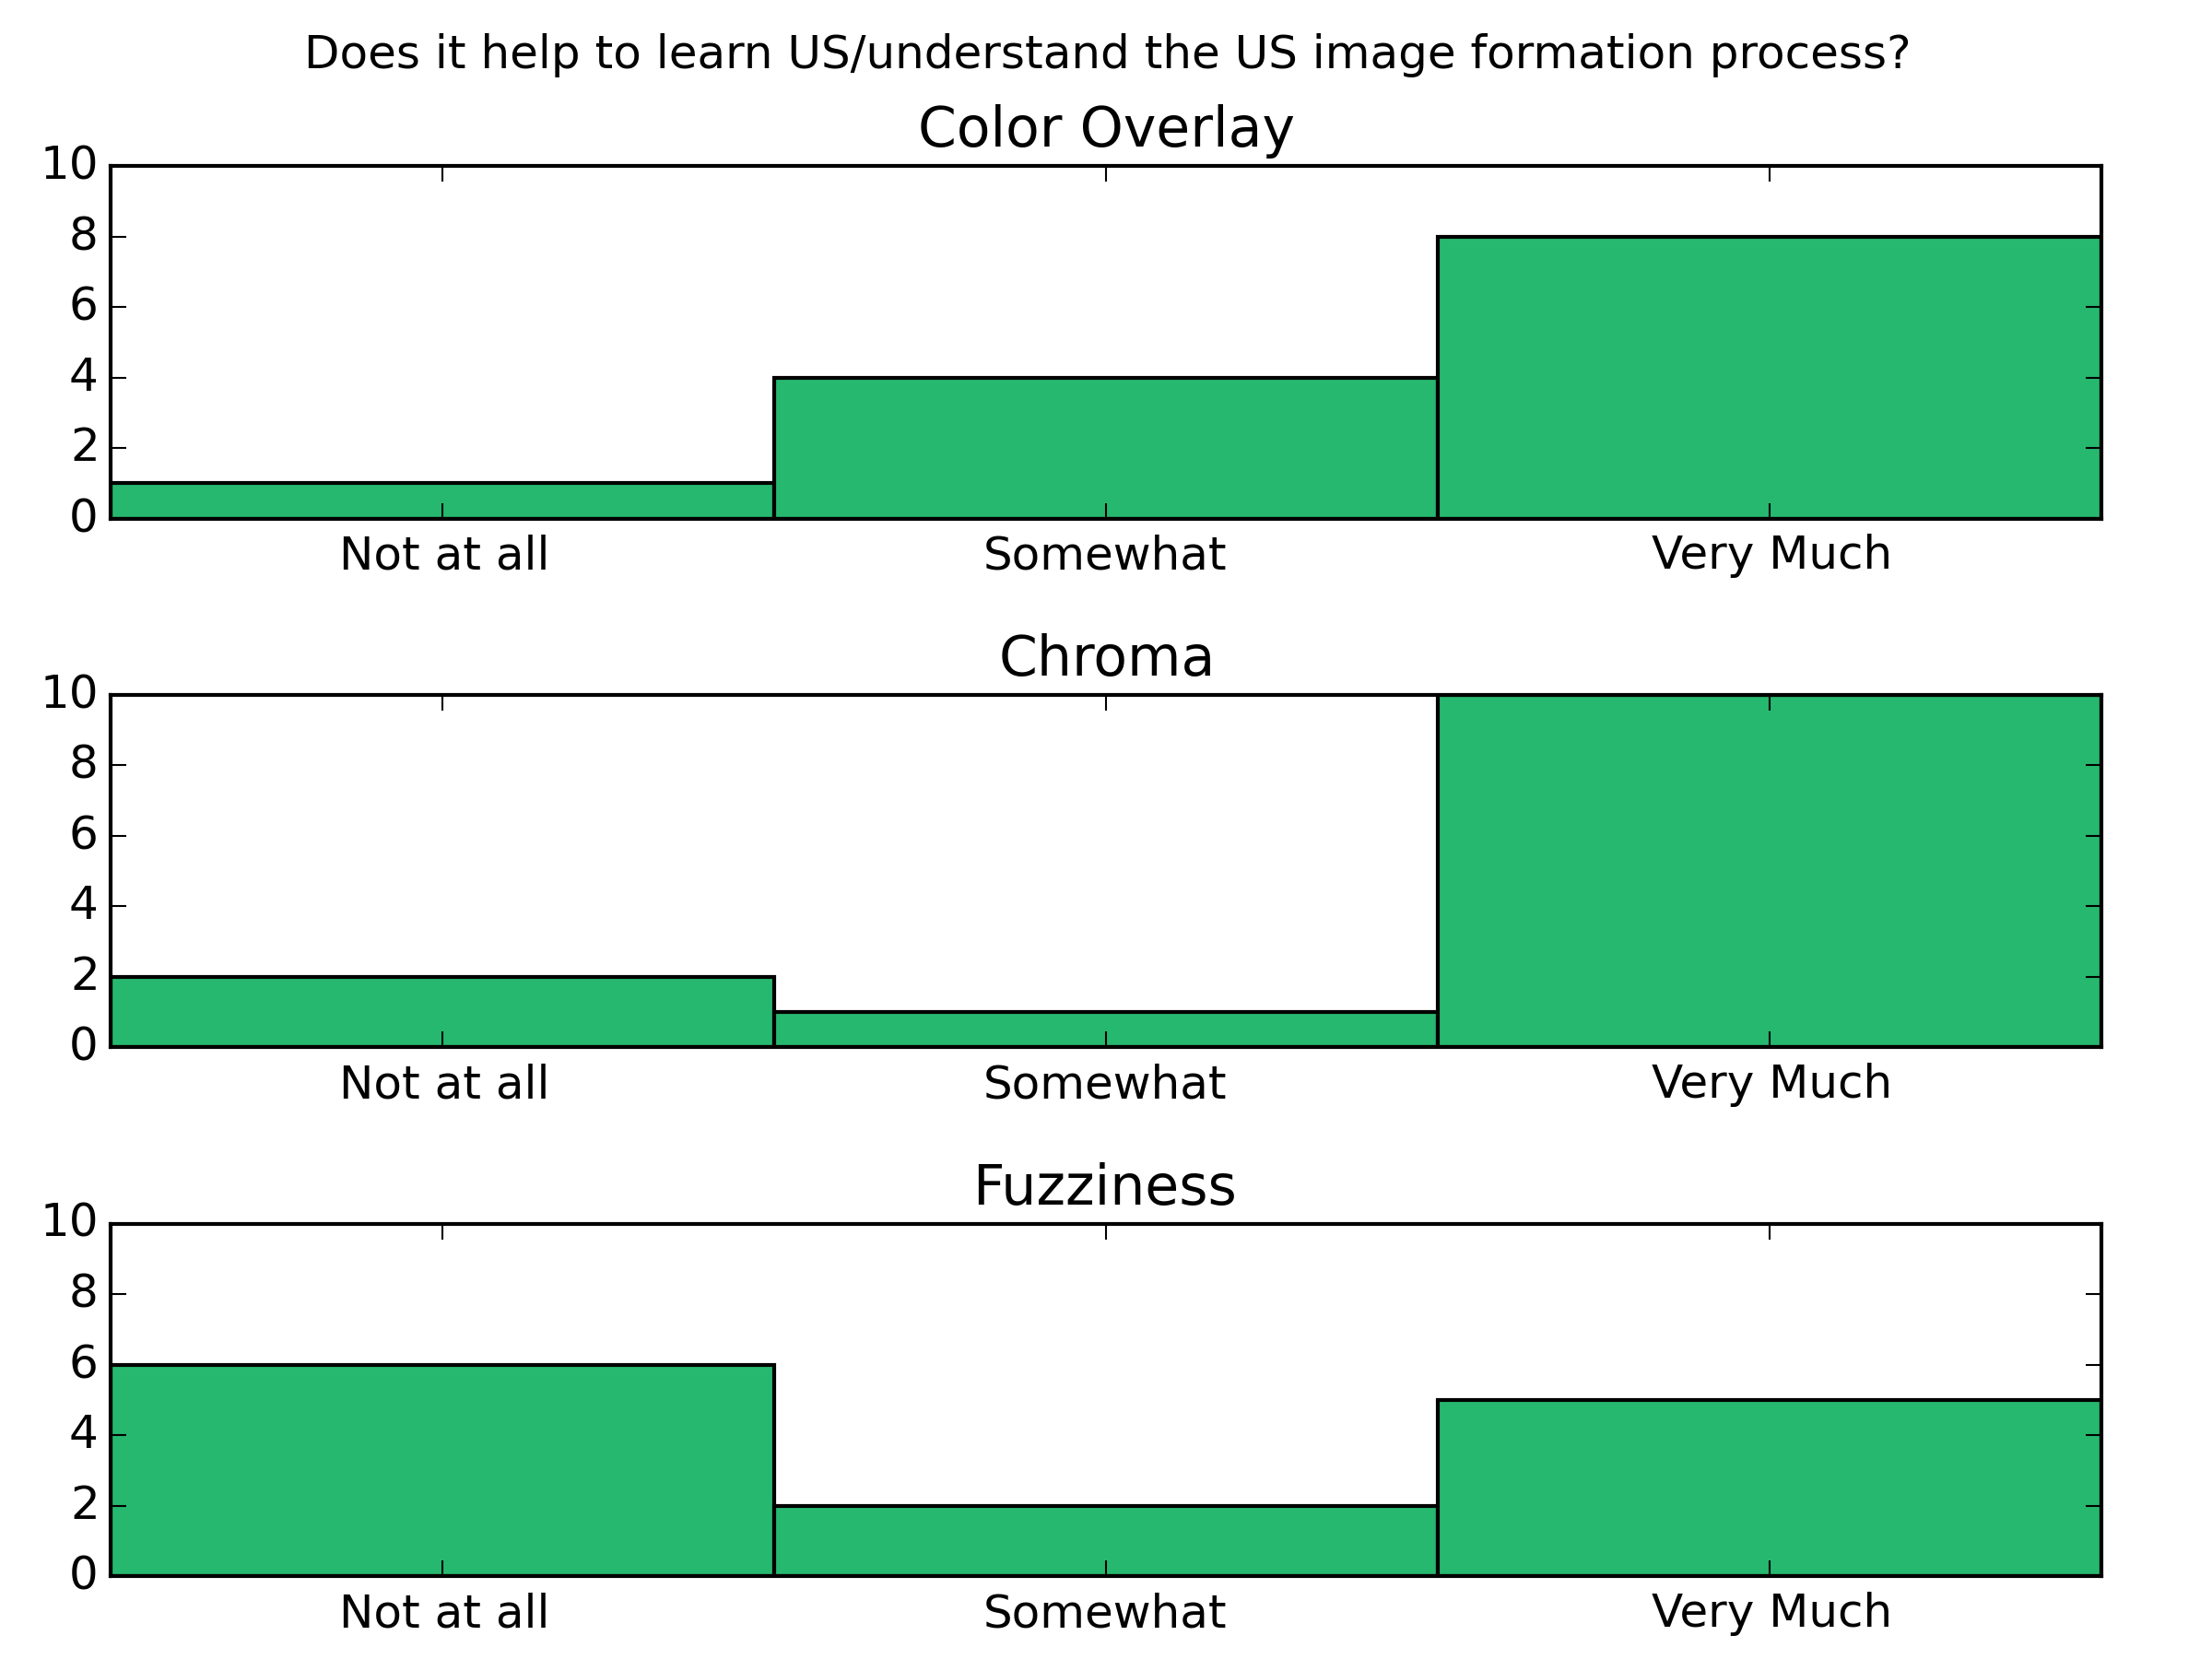
\includegraphics[width=0.49\linewidth]{{figures/cmvis/evaluation/helpful_to_learn_us}.png}
	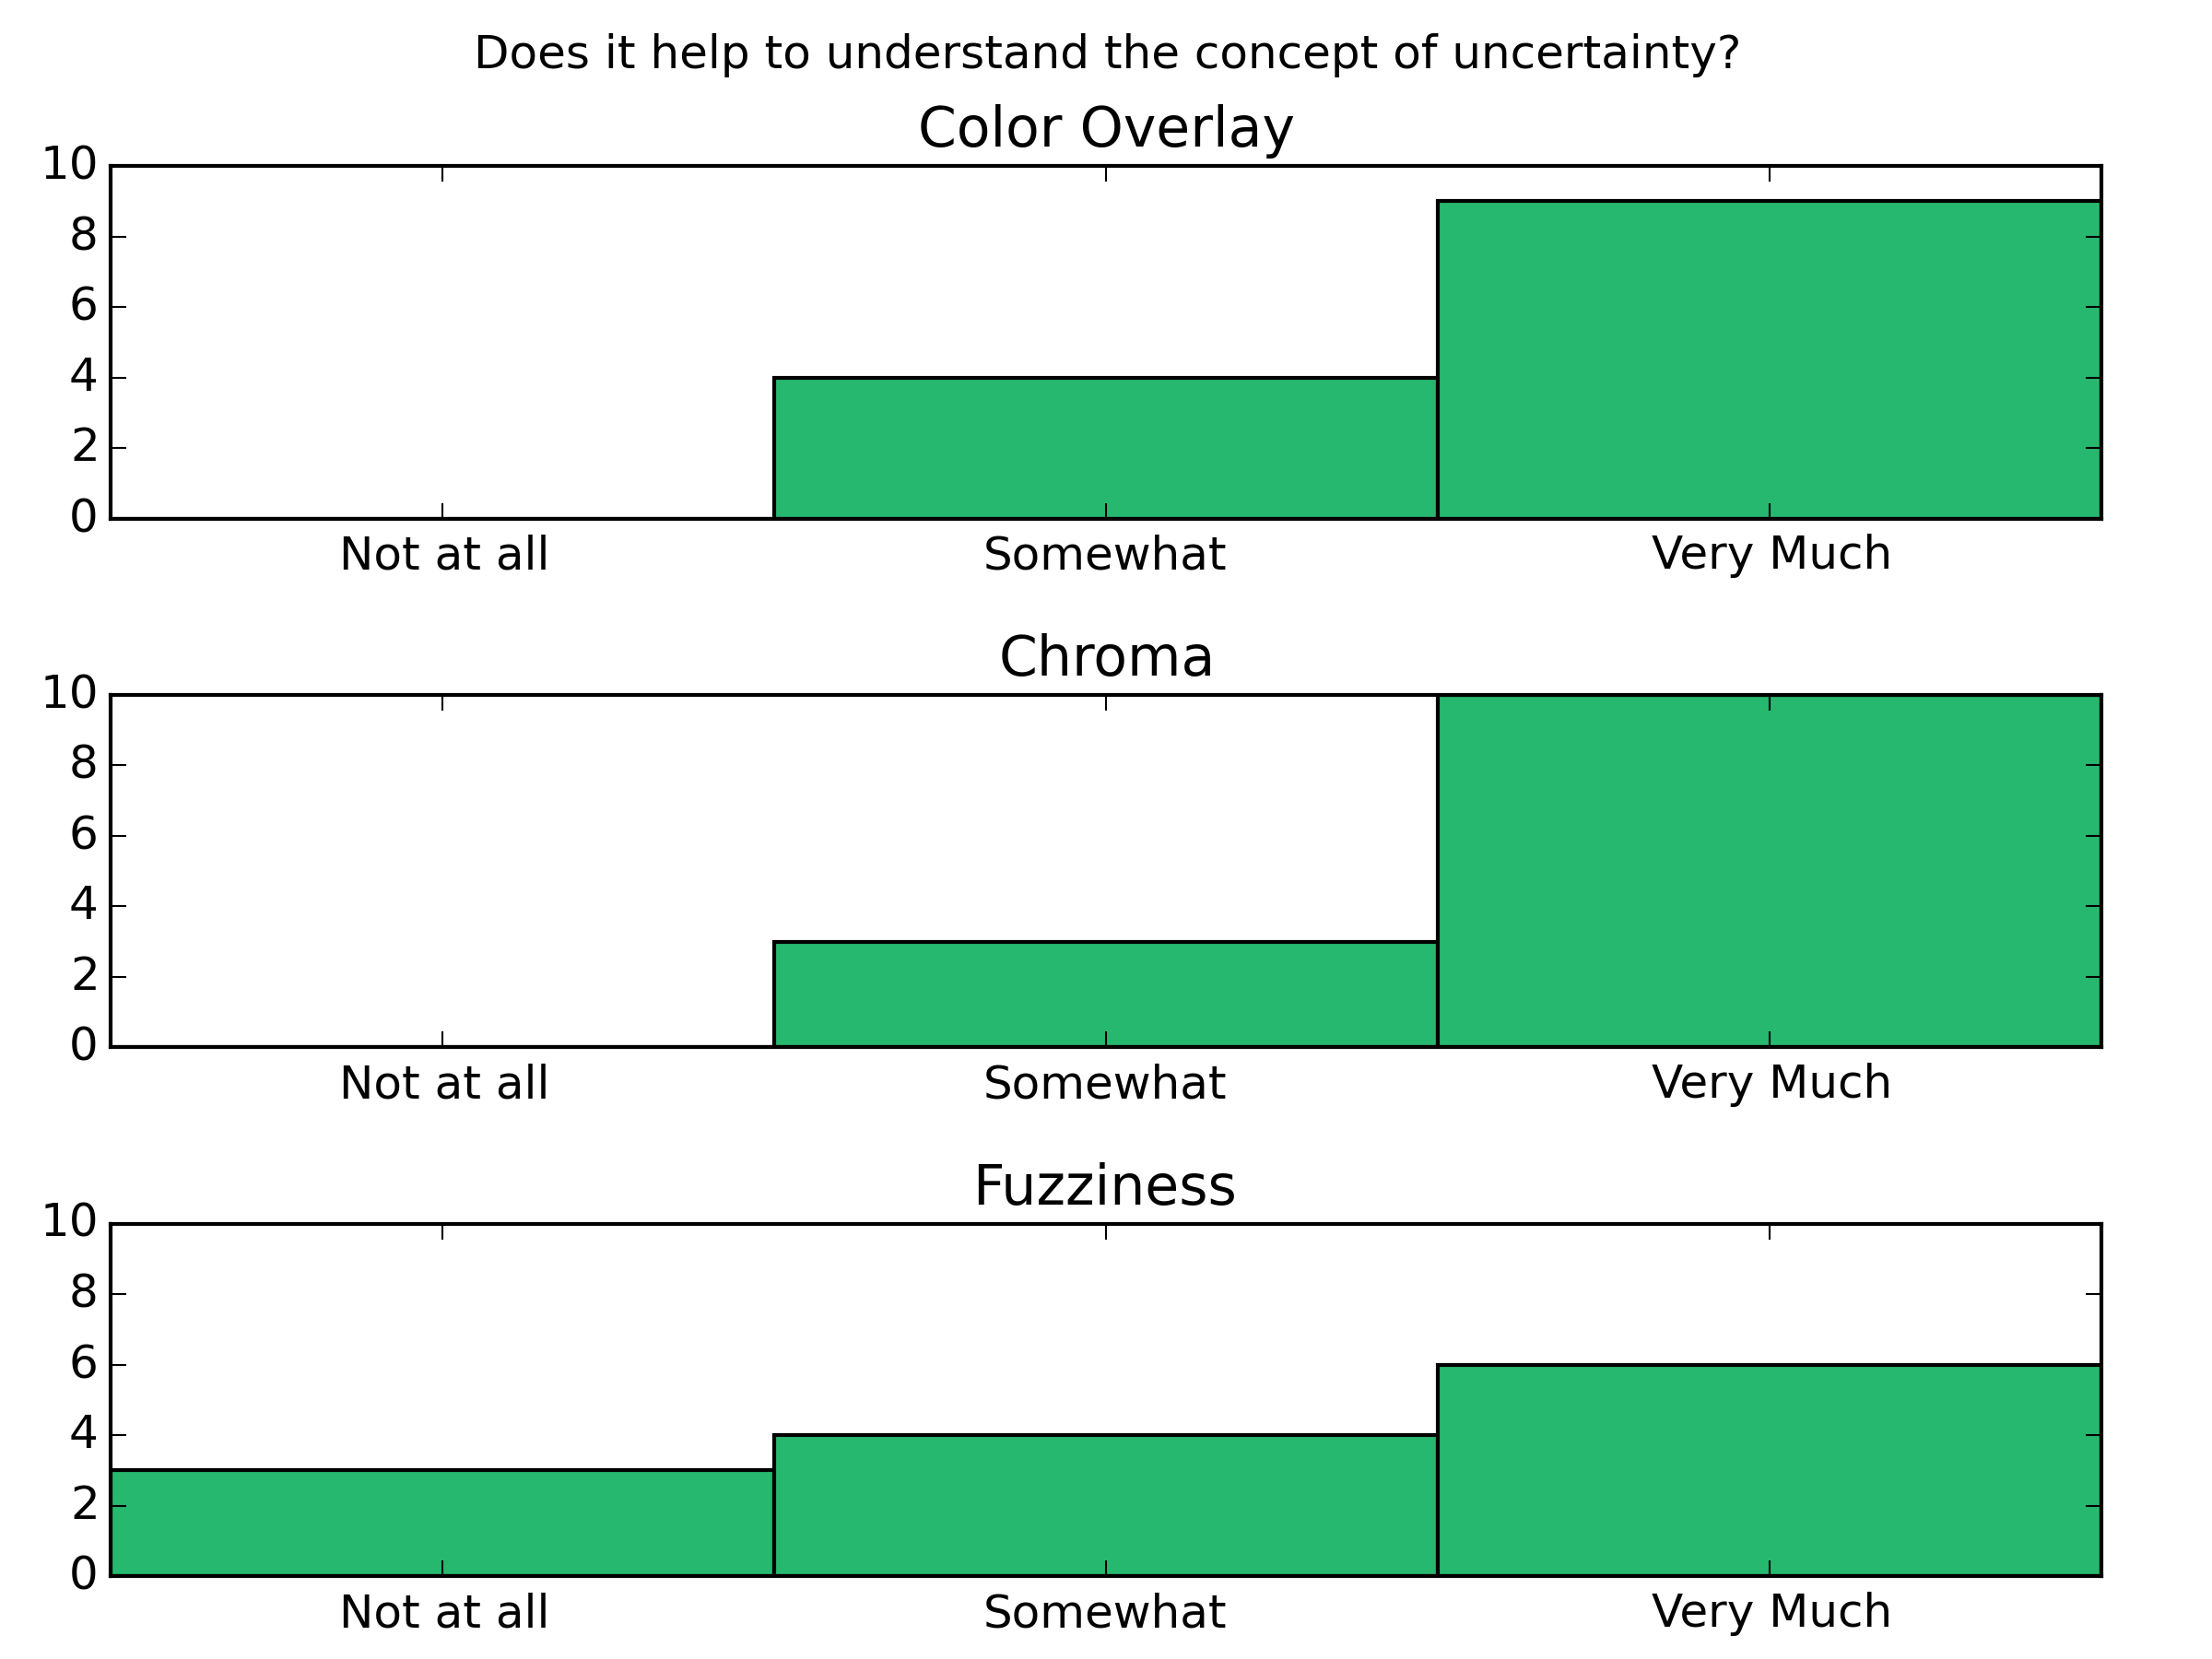
\includegraphics[width=0.49\linewidth]{{figures/cmvis/evaluation/helpful_to_understand_uncertainty}.png}
	\caption{
		User study results on the educational value of our technique to ultrasound novices.
		Almost all test subjects appreciate the added uncertainty visualization and confirm that it helps them with understanding the ultrasound image formation process and getting a better understanding of uncertainty in B-mode imaging.
	}
	\label{fig:cmvis:study-results-novices1}
\end{figure}

After the experiment, the test subjects additionally answered a short questionnaire on different aspects of die presented visualization schemes.
In the first set of questions we asked the students whether they generally appreciate the additional information presented to them, whether it helps them to better understand the ultrasound image formation process and whether it helps them with understanding the concept of uncertainty in B-mode images.
The results (cf. Figure \ref{fig:cmvis:study-results-novices1}) indicate a general level of appreciation for our presented techniques, since especially the color overlay method got very positive results.
In the second set of questions the students were asked to asses the intuitiveness of the presented visualizations and whether our technique helps them in finding anatomical structures faster.
As shown in Figure \ref{fig:cmvis:study-results-novices2}, ultrasound novices find the colorful visualizations much more intuitive than the fuzziness mapping.
However, only a few students found the presented visualizations helpful to find target anatomies faster.
Interestingly, fuzziness mapping yielded an overall worse response in the questionnaire, as many students considered this scheme as not helpful for diagnosis nor intuitive to read.
This result is particularly interesting as it contradicts the quantitative results of Table \ref{tbl:cmvis:timing-results}.

\begin{figure}[ht]
	\centering
	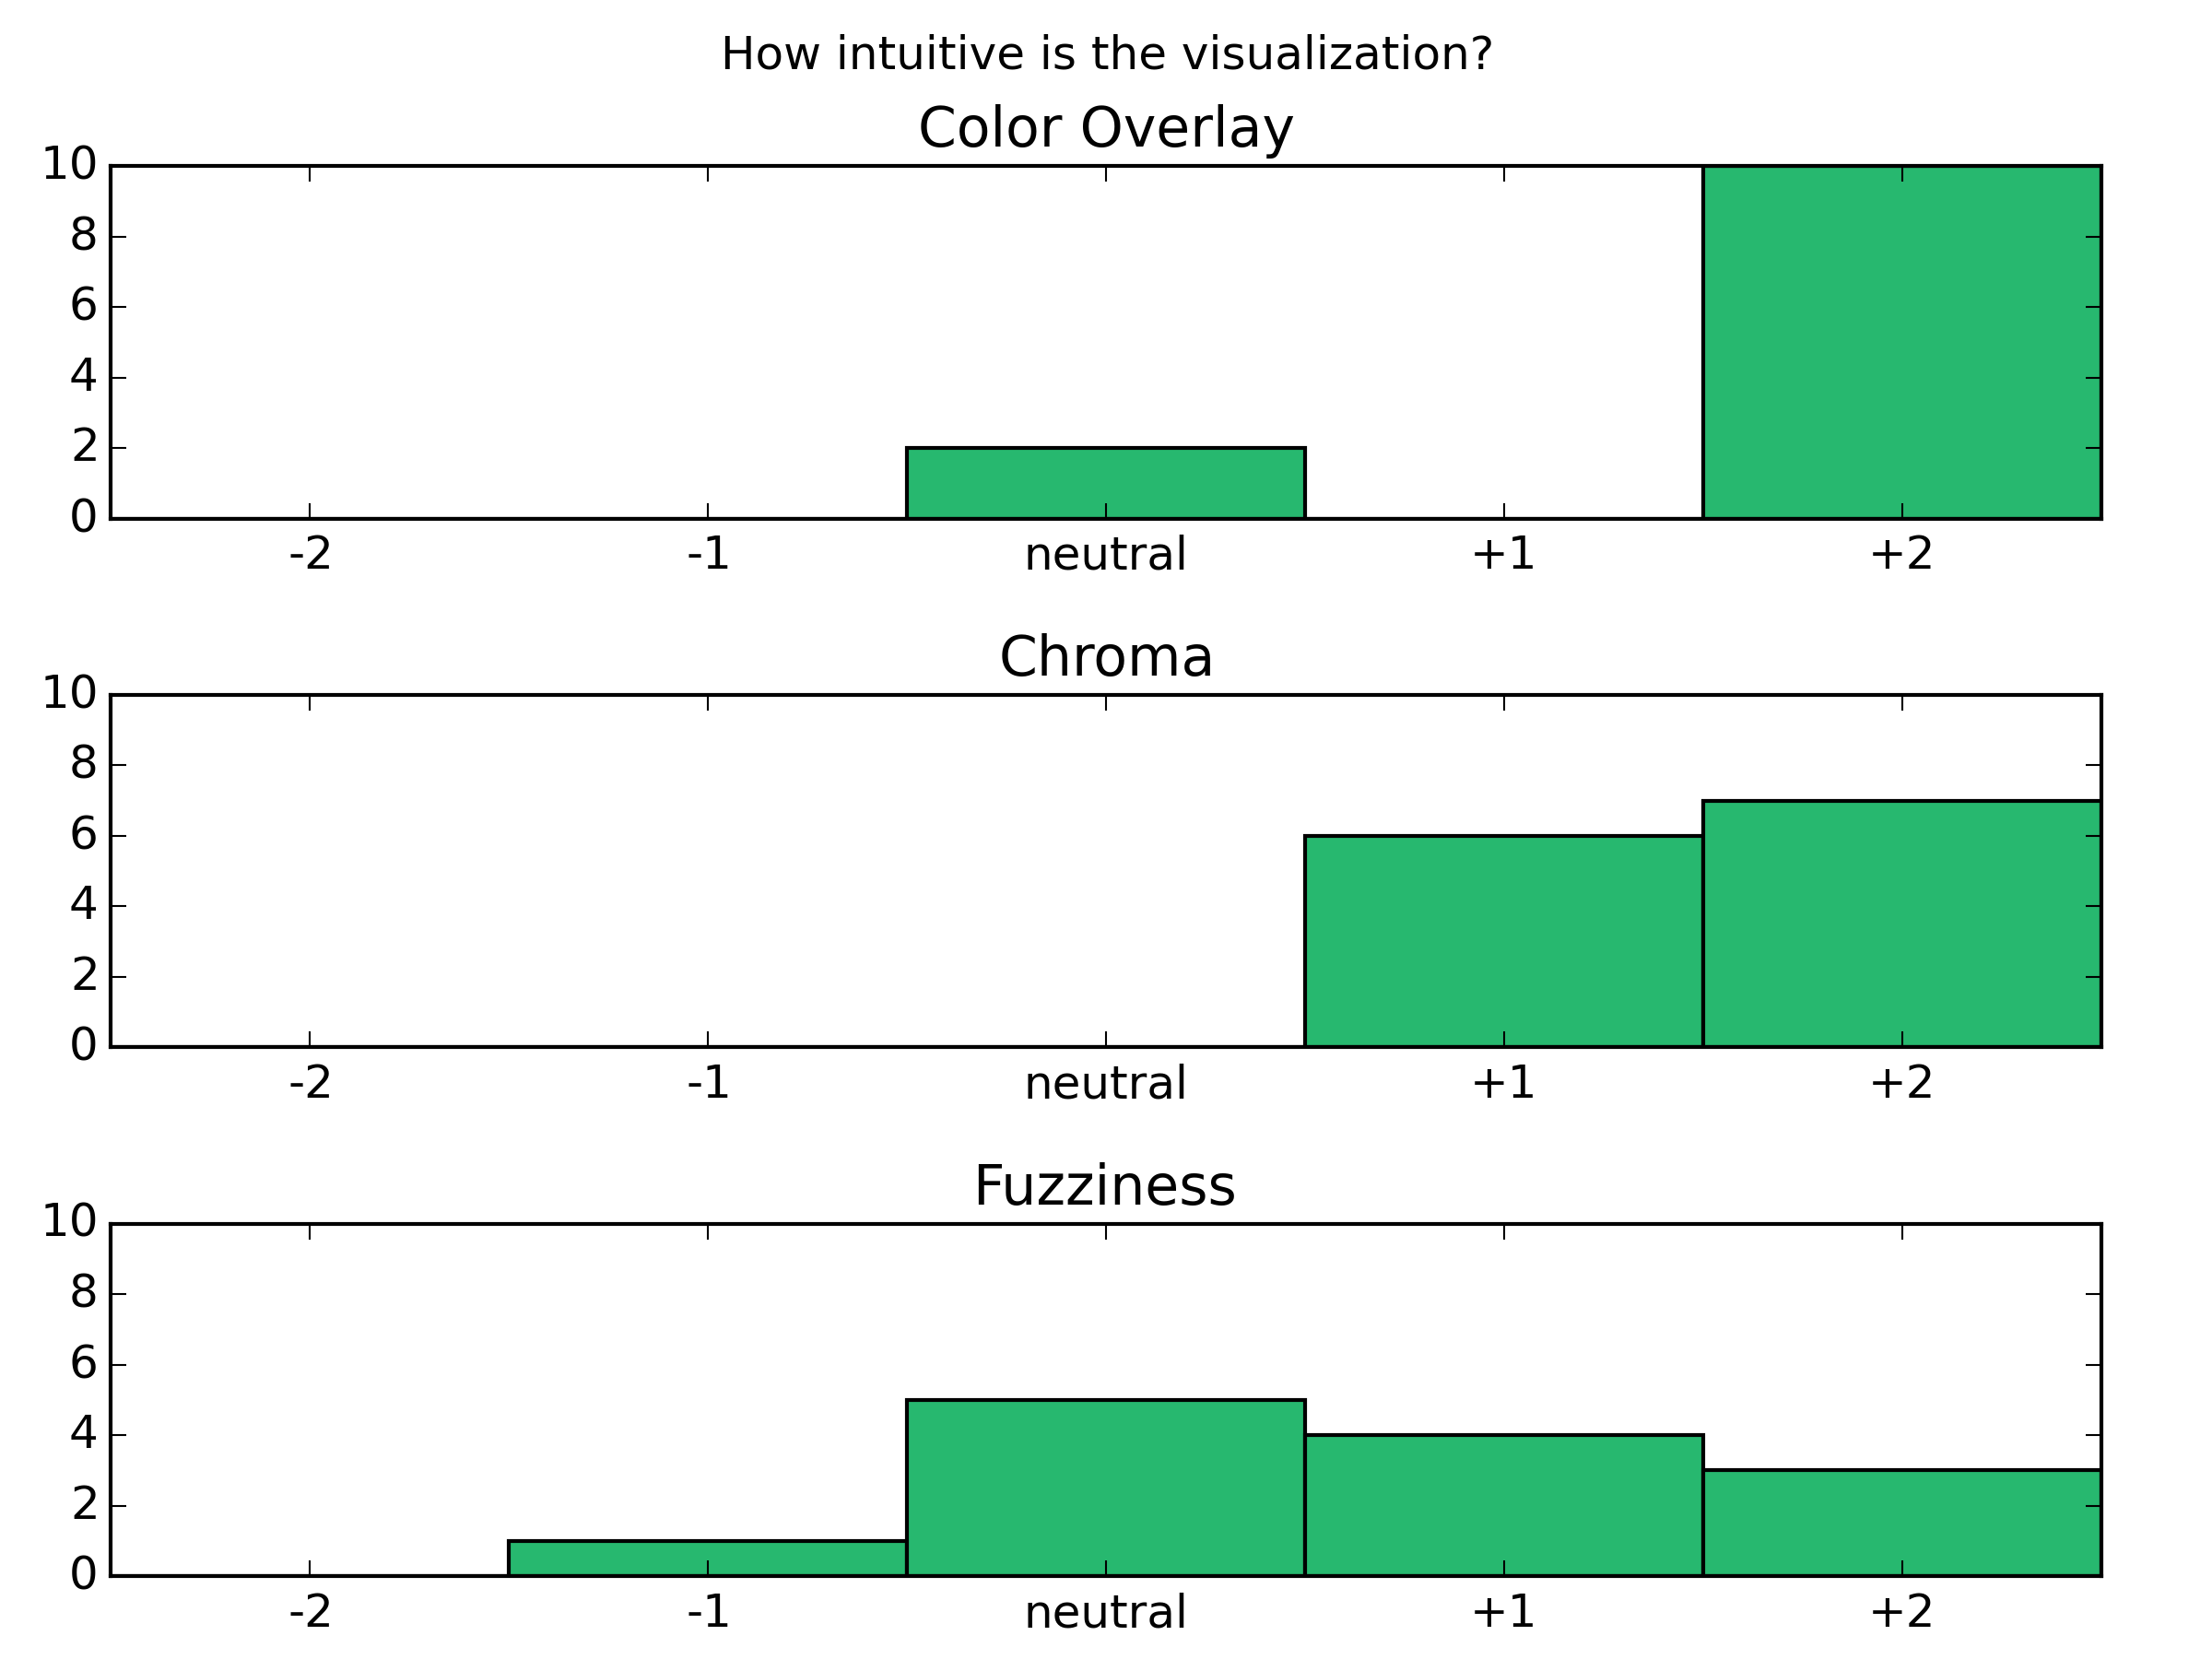
\includegraphics[width=0.49\linewidth]{{figures/cmvis/evaluation/intuitiveness}.png}
	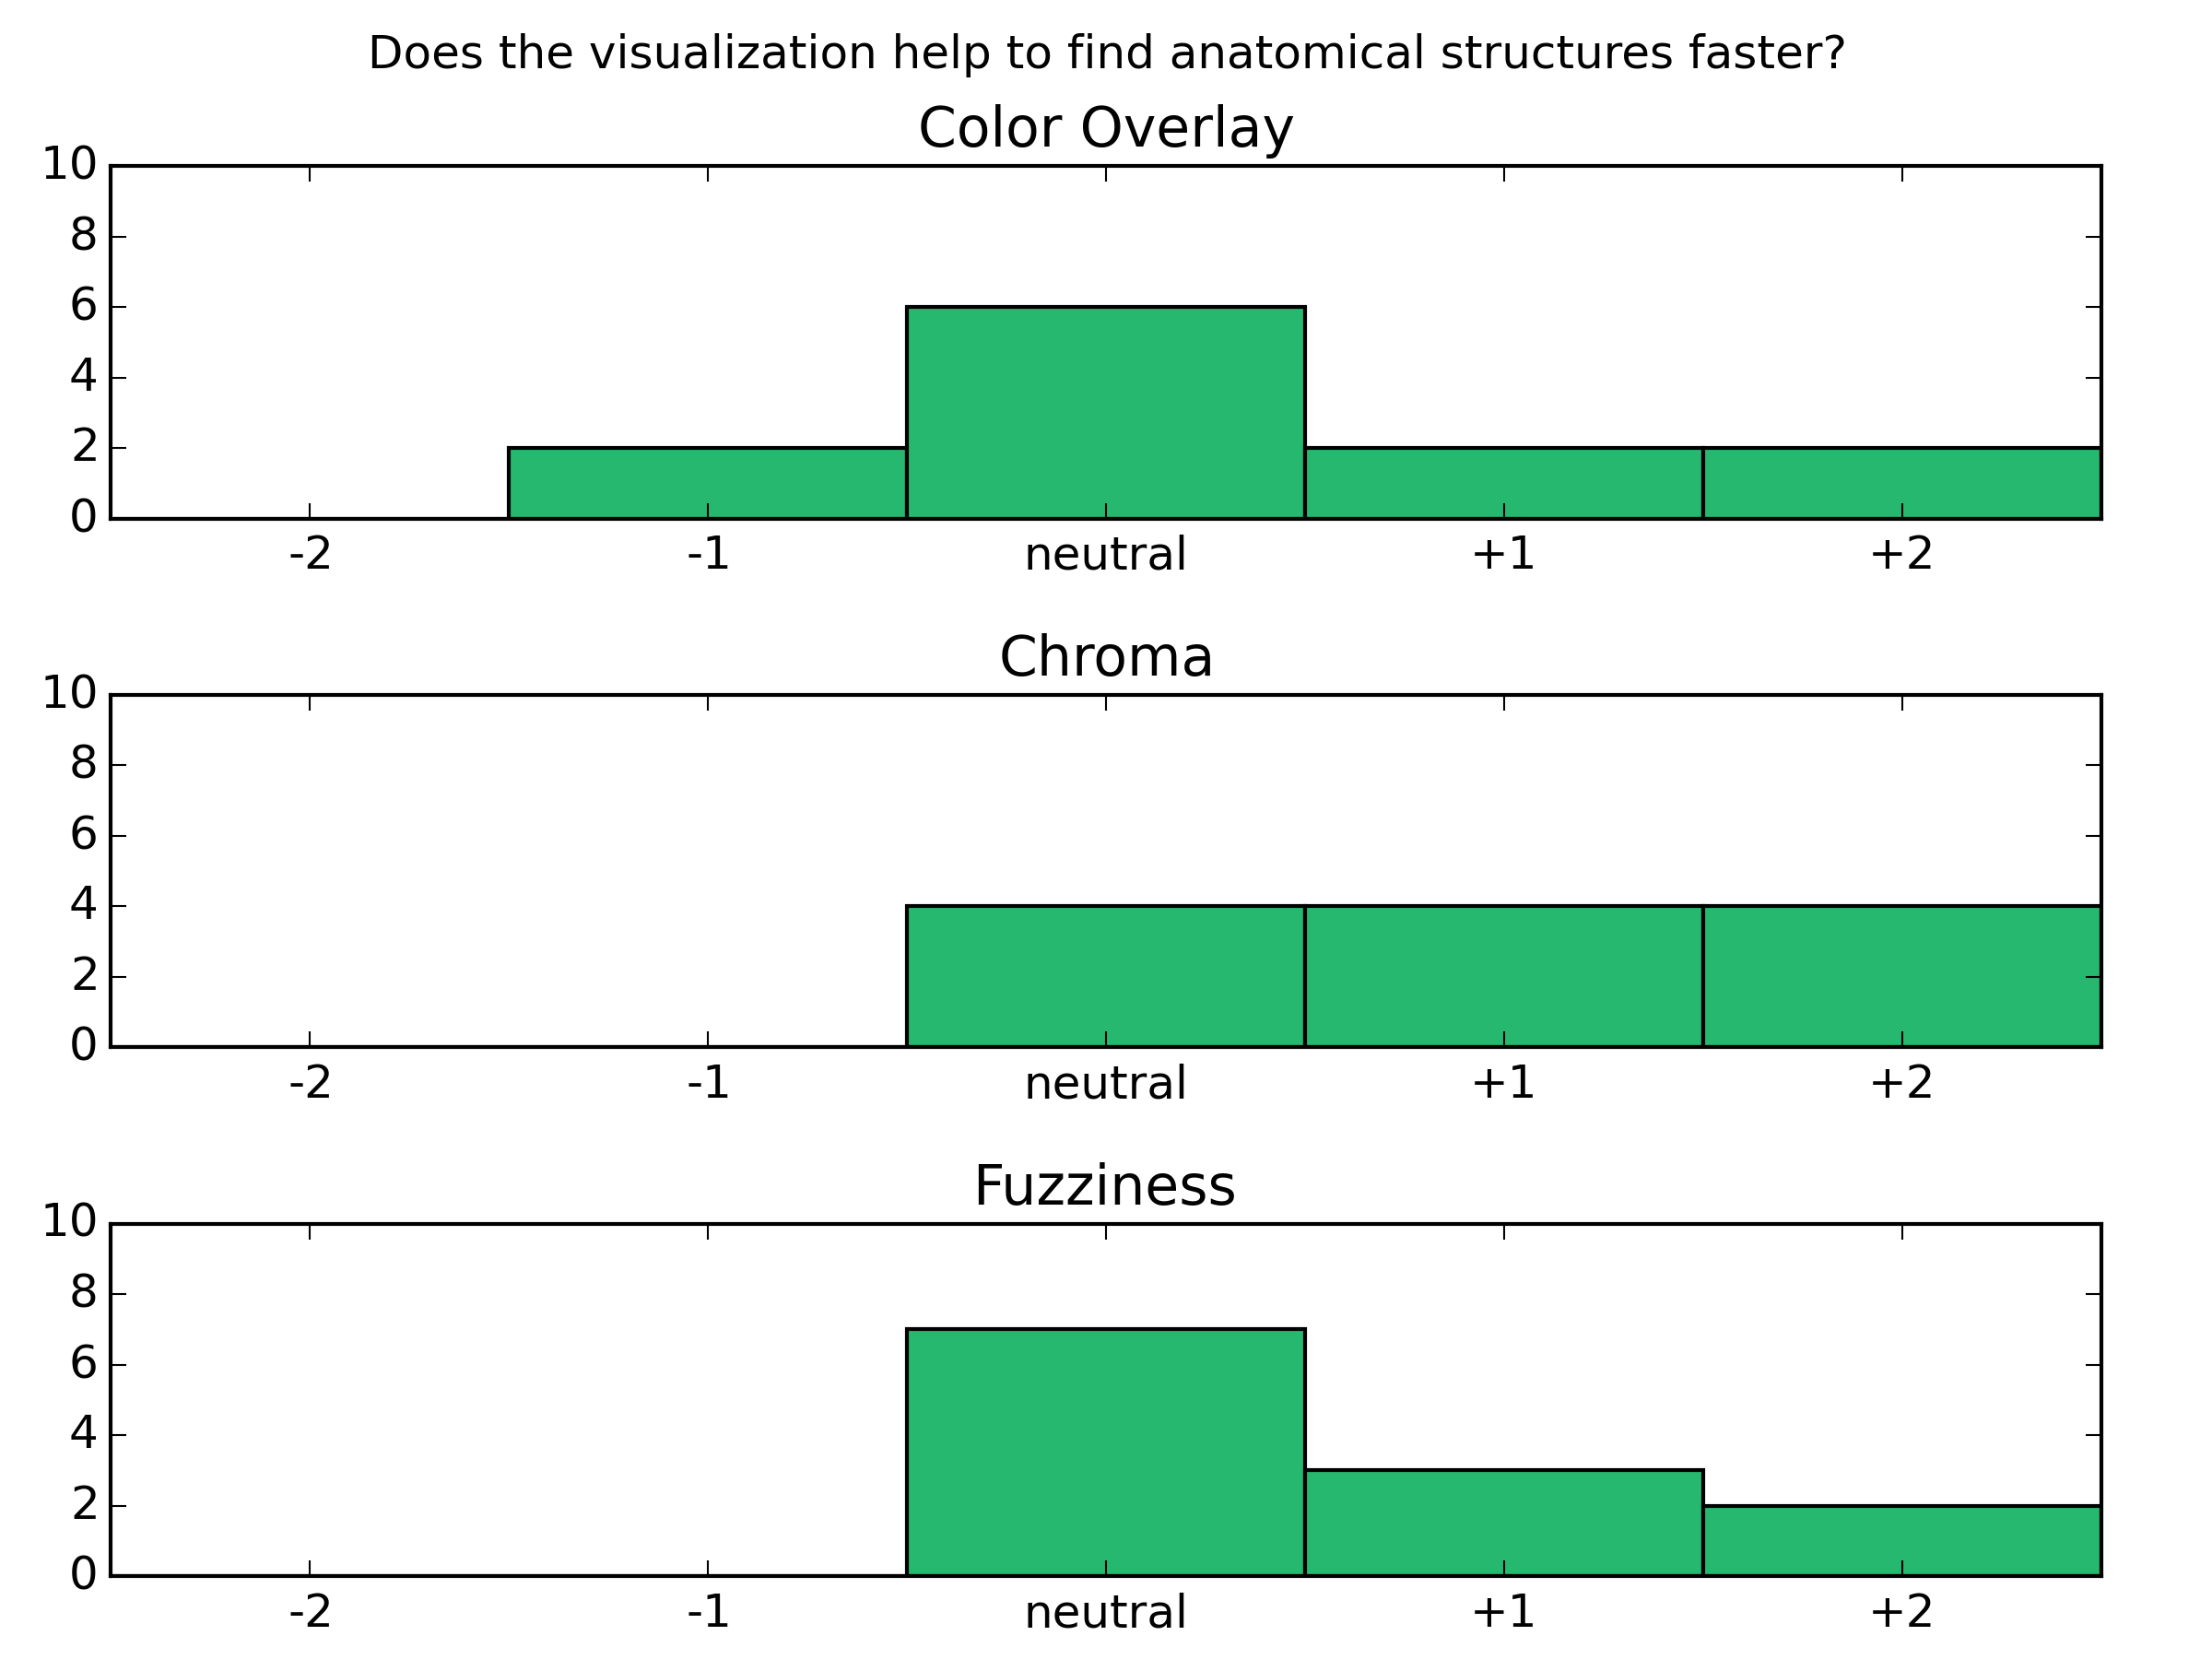
\includegraphics[width=0.49\linewidth]{{figures/cmvis/evaluation/helpful_to_find_anatomy}.png}
	\caption{
		User study results on the perception and clinical value for ultrasound novices on a 5-point Likert scale.
		While there is no clear favorite visualization scheme, a bias towards the colorful mappings is present.
		Furthermore, some students said that the added information helps them with finding target anatomical structures faster.
	}
	\label{fig:cmvis:study-results-novices2}
\end{figure}



\subsection{User Study with Ultrasound Experts}
In a second user study, we presented our system to expert sonographers in order to evaluate the clinical significance of real-time ultrasound uncertainty visualization.
Therefore we applied our visualization schemes to clinical data of abdominal ultrasound and presented the results to 7 experts (5 clinicians, 2 senior researchers).
We presented them two patient abdominal ultrasound sequences of three different anatomies (liver, kidney, spleen) and asked them about perception, clinical value as well as whether our techniques assist in finding the optimal acoustic window. 
Since, for clinical usage, we do not want to hide information in the B-mode image, we evaluated only mapping to chroma and mapping to fuzziness.

\begin{figure}[ht]
	\centering
	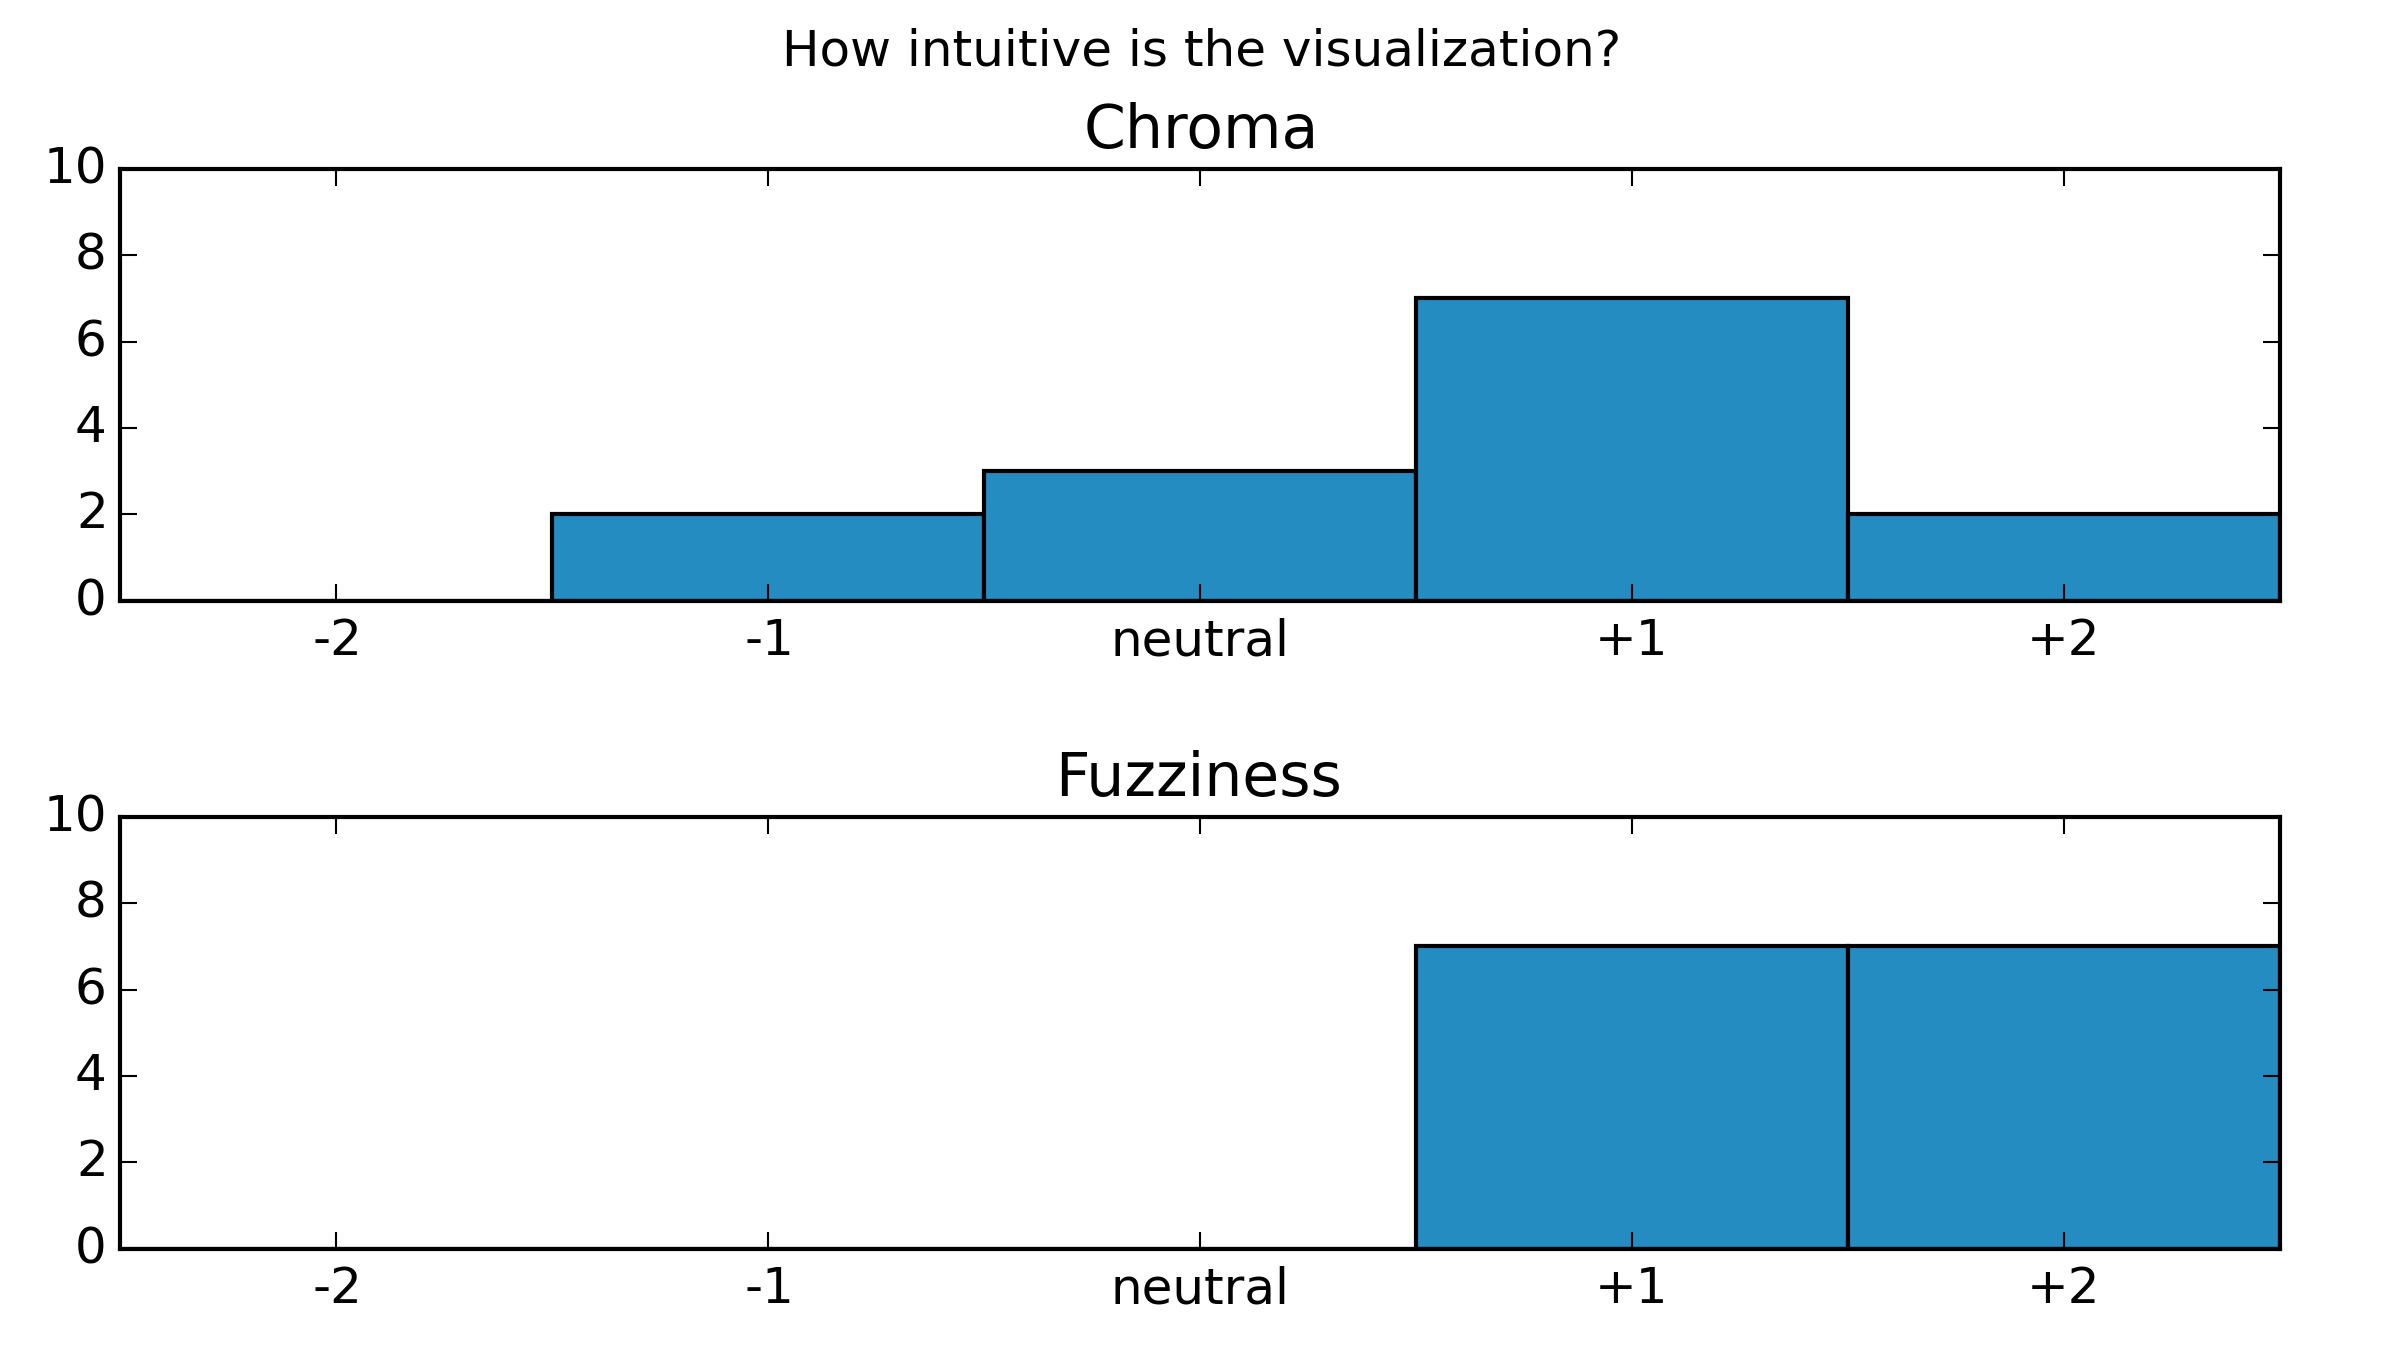
\includegraphics[width=0.49\linewidth]{{figures/cmvis/evaluation/expert_uncertainty_perception}.png}
	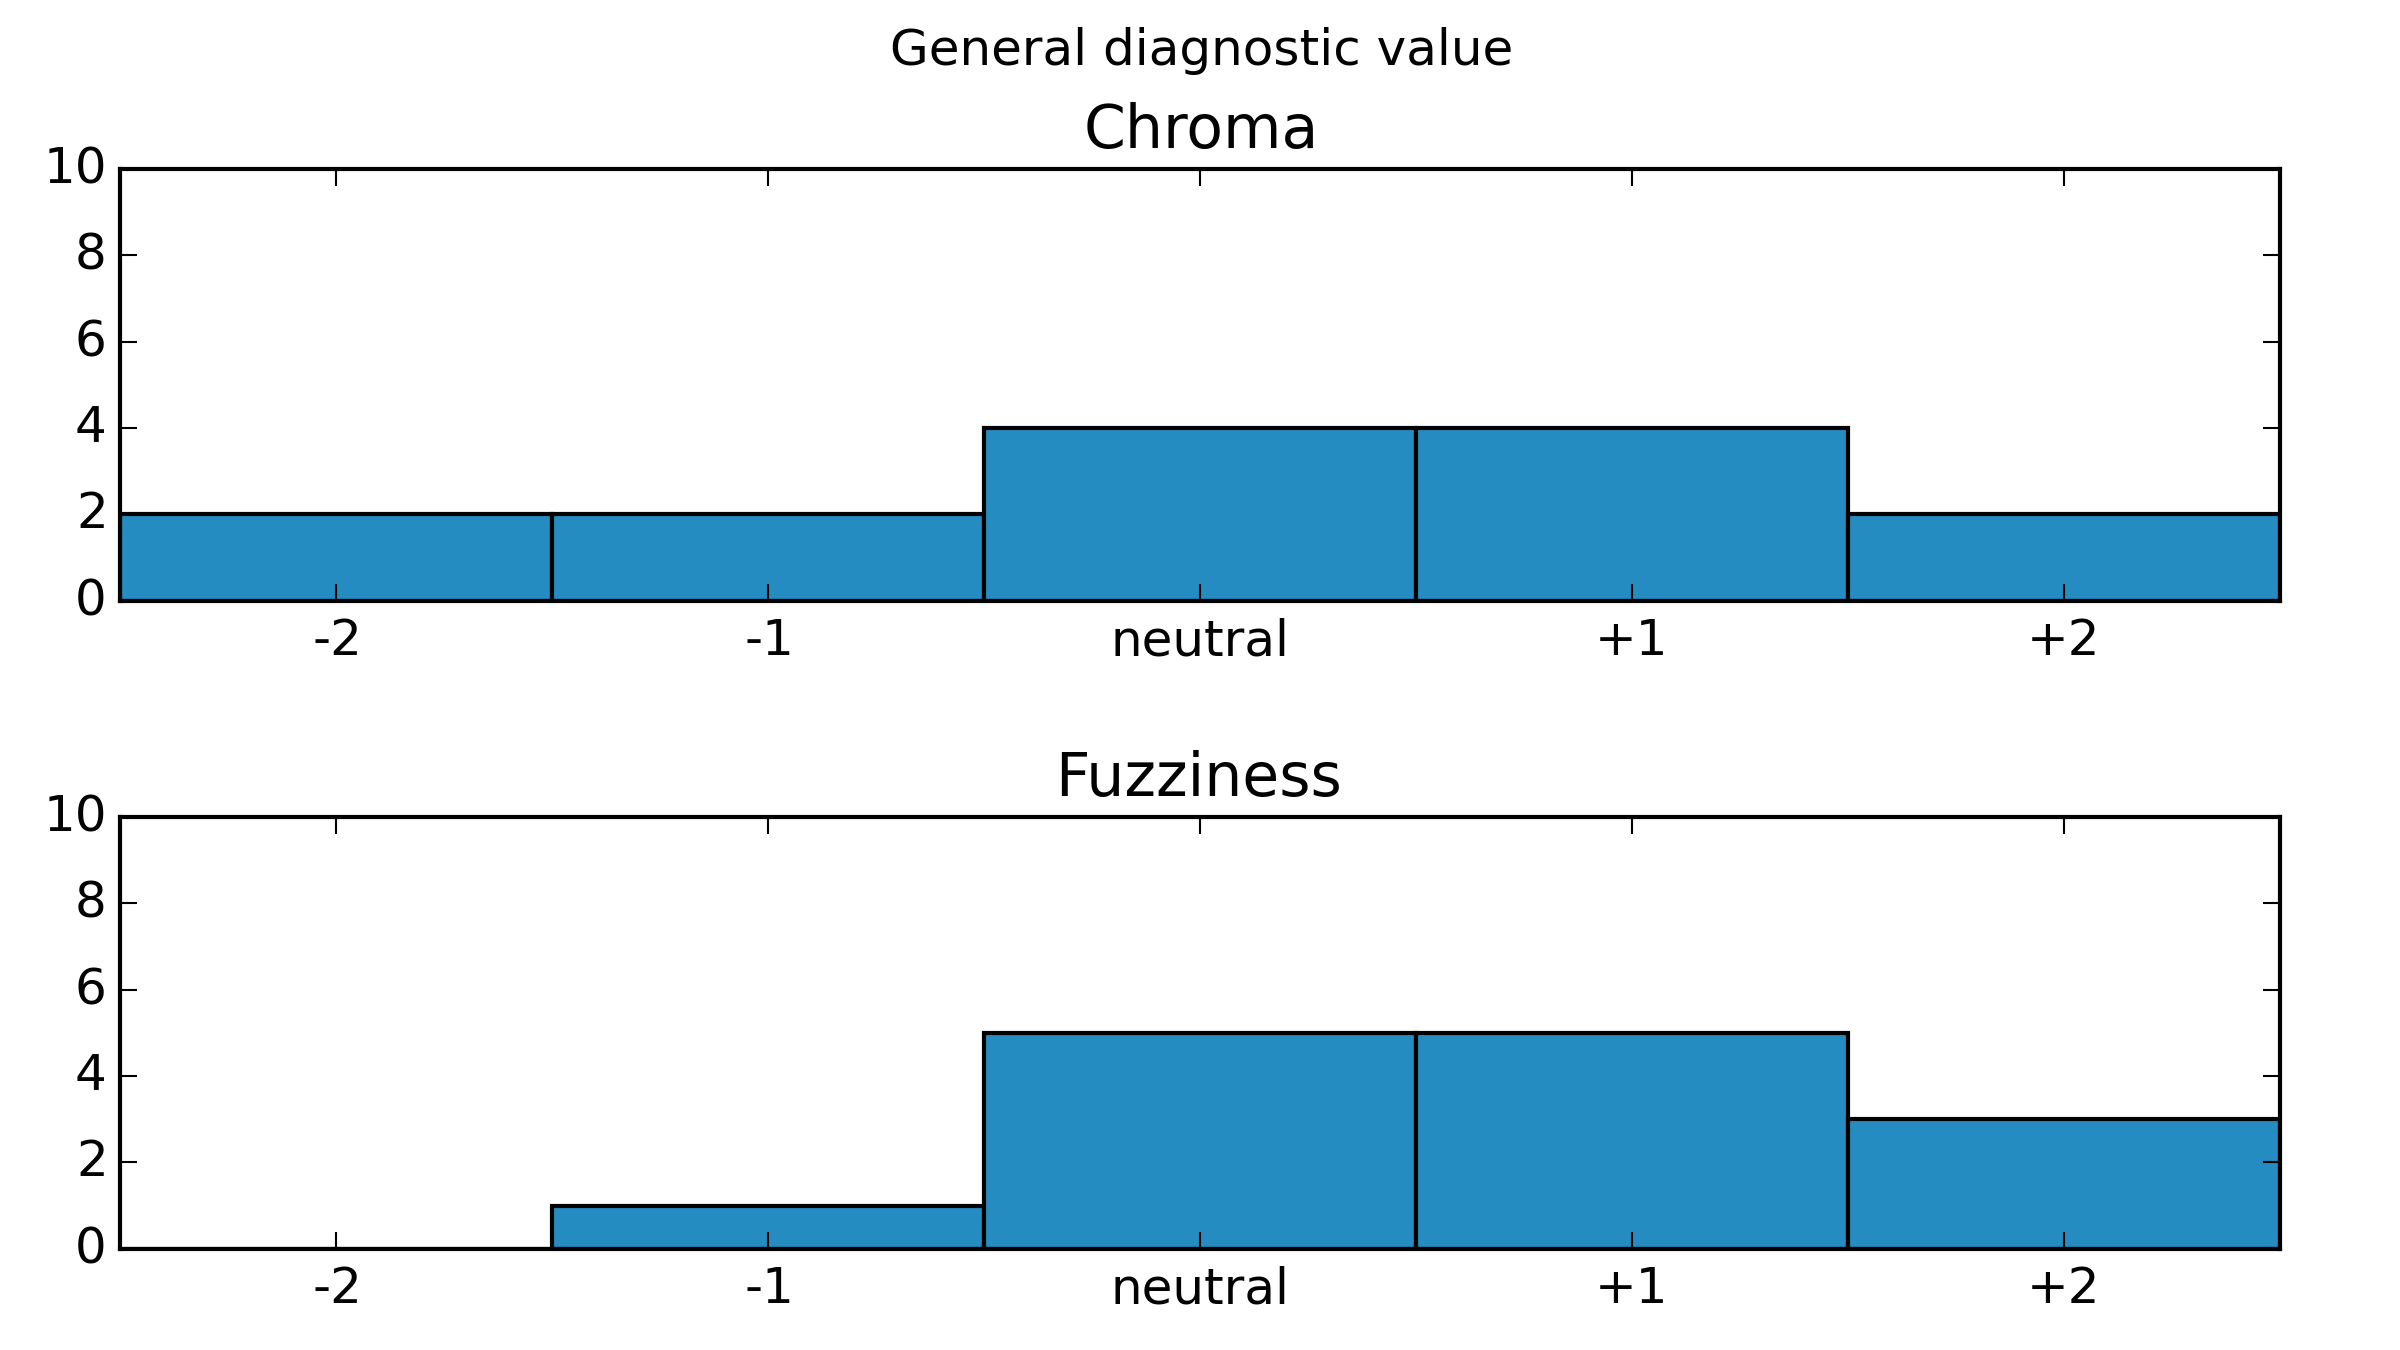
\includegraphics[width=0.49\linewidth]{{figures/cmvis/evaluation/expert_diagnostic_value}.png}
	\caption{
		Questionnaire results on \textbf{expert sonographers' uncertainty perception}. Each question was answered independently for the two different sequences. Therefore, there are 14 answers in total.
		}
	\label{fig:cmvis:expert-perception}
\end{figure}

As shown in Figure \ref{fig:cmvis:expert-perception}, the expert sonographers clearly prefer mapping to fuzziness over mapping to chroma.
The results on general diagnostic value are quite mixed.
While there is a slight positive response for the gray scale fuzziness mapping, the chroma mapping performs rather bad in this regard.
This discrepancy compared to ultrasound novices is probably due to the fact that experts got used to the monochrome appearance of B-mode ultrasound over the years.
Thus, they prefer a visualization scheme that keeps the image in its original gray scale domain.

In addition to asking about the general diagnostic value, we also asked more specific questions regarding the clinical significance.
Here, the study shows significant improvements compared to the default visualization in today's ultrasound devices (Table \ref{tbl:cmvis:results}).
The clinicians reported that seeing the amount of uncertainty dynamically adapting to the ultrasound view provides them with a very strong feedback on the image quality and its credibility.
Here, 6 out of 7 stated that our uncertainty visualization helps with the correct interpretation of the images and also 6 out of 7 participants confirmed that the proposed real-time visualization schemes assists in optimizing the acoustic window.
One clinician found that the computed Confidence Map was unexpected in one of the sequences and therefore confused him with the correct interpretation of the image. 
Nevertheless, he stated that the technique was helpful for optimizing the acoustic window.
One other clinician confirmed the uncertainty visualization to be helpful for the correct interpretation but had doubts that it helps with optimizing the acoustic window.

\begin{table}[th]
	\centering
	\begin{tabu} to 0.9\linewidth {>{\bfseries}m{64mm} C C}
		\toprule
		\quad                             & \bfseries Yes & \bfseries No \\
		\midrule
		Helps with Correct Interpretation & ${86\%}$      & $14\%$       \\
		Helps Optimizing Acoustic Window  & ${86\%}$      & $14\%$       \\
		\bottomrule
	\end{tabu}
	\caption{Results on \textbf{expert sonographers evaluating the clinical value}.}
	\label{tbl:cmvis:results}
\end{table}


\section{Conclusion}
\label{sec:cmvis:conclusion}
In this chapter we introduced a novel \SYN{paradigm} to 2D ultrasound visualization.
Instead of only showing the plain B-mode image, we augment it with additional uncertainty information based on the estimated per-pixel signal attenuation.
Though different works have introduced the concept of uncertainty to ultrasound image processing, such information has never been exposed to the user.

To do so, we build upon the previously introduced technique of real-time uncertainty estimation (cf. Chapter \ref{chap:cudacm}) and fuse Confidence Maps with their original B-mode image.
Targeting both educational and clinical applications, we present three individually designed visualization schemes.
After implementing a fully working system, we ran two user studies \SYN{on/with} both ultrasound novices and experts sonographers.
The results clearly show the benefit of our technique for educational purposes as the added feedback on the signal attenuation helps students interactively learn how the ultrasound image formation process works.
Also most clinicians value the additional information since it can help them with optimizing the acoustic window on target anatomies.
